\DocumentMetadata{%
 %  uncompress, %only for debugging!!
  pdfversion=2.0,
  testphase={phase-II, tabular, graphic}%
 % testphase={phase-II,math, tabular, graphic}% TOC Does not work
   % testphase={phase-III,math}% TOC works
}
\tagpdfsetup{activate, tabsorder=structure}
% Use the following to fix bug in November 2023 download of LaTeX
\ExplSyntaxOn
\cs_generate_variant:Nn\__tag_prop_gput:Nnn{cnx}
\ExplSyntaxOff
\documentclass[11pt,
  english,
  letterpaper,
]{article}
\usepackage{sa4ss}
\usepackage{amsmath,amssymb,array}
\usepackage{booktabs}

% From tagged-template.latex
\usepackage{lmodern}
\usepackage{ifxetex,ifluatex}
\ifnum 0\ifxetex 1\fi\ifluatex 1\fi=0 % if pdftex
  \usepackage[T1]{fontenc}
  \usepackage[utf8]{inputenc}
  \usepackage{textcomp} % provide euro and other symbols
\else % if luatex or xetex
  \usepackage{unicode-math}
  \defaultfontfeatures{Scale=MatchLowercase}
  \defaultfontfeatures[\rmfamily]{Ligatures=TeX,Scale=1}
\fi

% Use upquote if available, for straight quotes in verbatim environments
\IfFileExists{upquote.sty}{\usepackage{upquote}}{}
\IfFileExists{microtype.sty}{% use microtype if available
  \usepackage[]{microtype}
  \UseMicrotypeSet[protrusion]{basicmath} % disable protrusion for tt fonts
}{}
\makeatletter
\@ifundefined{KOMAClassName}{% if non-KOMA class
  \IfFileExists{parskip.sty}{%
    \usepackage{parskip}
  }{% else
    \setlength{\parindent}{0pt}
    \setlength{\parskip}{6pt plus 2pt minus 1pt}}
}{% if KOMA class
  \KOMAoptions{parskip=half}}
\makeatother
\usepackage{xcolor}
\IfFileExists{xurl.sty}{\usepackage{xurl}}{} % add URL line breaks if available
\hypersetup{
  pdftitle={Status of Copper Rockfish (Sebastes caurinus) along the California North of Pt. Conception U.S. West coast in 2022},
  pdflang={en},
  hidelinks,
  pdfcreator={LaTeX via pandoc}}
\urlstyle{same} % disable monospaced font for URLs
\usepackage{longtable}
% Correct order of tables after \paragraph or \subparagraph
\usepackage{etoolbox}
\makeatletter
\patchcmd\longtable{\par}{\if@noskipsec\mbox{}\fi\par}{}{}
\makeatother
% Allow footnotes in longtable head/foot
\IfFileExists{footnotehyper.sty}{\usepackage{footnotehyper}}{\usepackage{footnote}}
\makesavenoteenv{longtable}
\usepackage{graphicx}
\makeatletter
\def\maxwidth{\ifdim\Gin@nat@width>\linewidth\linewidth\else\Gin@nat@width\fi}
\def\maxheight{\ifdim\Gin@nat@height>\textheight\textheight\else\Gin@nat@height\fi}
\makeatother
% Scale images if necessary, so that they will not overflow the page
% margins by default, and it is still possible to overwrite the defaults
% using explicit options in \includegraphics[width, height, ...]{}
\setkeys{Gin}{width=\maxwidth,height=\maxheight,keepaspectratio}
% Set default figure placement to htbp
\makeatletter
\def\fps@figure{htbp}
\makeatother
\setlength{\emergencystretch}{3em} % prevent overfull lines
\providecommand{\tightlist}{%
  \setlength{\itemsep}{0pt}\setlength{\parskip}{0pt}}
\setcounter{secnumdepth}{5}
\ifxetex
  % Load polyglossia as late as possible: uses bidi with RTL langages (e.g. Hebrew, Arabic)
  \usepackage{polyglossia}
  \setmainlanguage[]{}
\else
  \usepackage[shorthands=off,main=english]{babel}
\fi

%Define cslreferences environment, required by pandoc 2.8
%https://github.com/rstudio/rmarkdown/issues/1649
\newlength{\csllabelwidth}
\setlength{\csllabelwidth}{3em}
\newlength{\cslhangindent}
\setlength{\cslhangindent}{1.5em}
% for Pandoc 2.8 to 2.10.1
\newenvironment{cslreferences}%
  {}%
  {\par}
% For Pandoc 2.11+
\newenvironment{CSLReferences}[2] % #1 hanging-ident, #2 entry spacing
 {% don't indent paragraphs
  \setlength{\parindent}{0pt}
  % turn on hanging indent if param 1 is 1
  \ifodd #1 \everypar{\setlength{\hangindent}{\cslhangindent}}\ignorespaces\fi
  % set entry spacing
  \ifnum #2 > 0
  \setlength{\parskip}{#2\baselineskip}
  \fi
 }%
 {}
\usepackage{calc}  % for \widthof, \maxof in minipage
\newcommand{\CSLBlock}[1]{#1\hfill\break}
\newcommand{\CSLLeftMargin}[1]{\parbox[t]{\csllabelwidth}{#1}}
\newcommand{\CSLRightInline}[1]{\parbox[t]{\linewidth - \csllabelwidth}{#1}\break}
\newcommand{\CSLIndent}[1]{\hspace{\cslhangindent}#1}


\providecommand{\tightlist}{%
  \setlength{\itemsep}{0pt}\setlength{\parskip}{0pt}}


\date{}
\newcommand{\trTitle}{Status of Copper Rockfish (\emph{Sebastes caurinus}) along the California North of Pt. Conception U.S. West coast in 2022}
\newcommand{\trYear}{2023}
\newcommand{\trMonth}{March}
\newcommand{\trAuthsLong}{truetruetrue}
\newcommand{\trAuthsBack}{Monk, M.H., C.R. Wetzel, J. Coates}
\newcommand{\trCitation}{
\begin{hangparas}{1em}{1}
\trAuthsBack{}. \trYear{}. \trTitle{}. \glsentrylong{pfmc}, Portland, Oregon. \pageref{LastPage}{}\,p.
\end{hangparas}}

\begin{document}

%%%%% Frontmatter %%%%%

% Footnote symbols in front matter
\renewcommand*{\thefootnote}{\fnsymbol{footnote}}

\small
\thispagestyle{empty}
\pagenumbering{roman}
\noindent
\begin{center}
\title{Status of Copper Rockfish (\emph{Sebastes caurinus}) along the California North of Pt. Conception U.S. West coast in 2022}
% \textnormal{\MakeTextUppercase{\trTitle{}}}
\vspace{1.5cm}
{\Large\textbf\newline{Status of Copper Rockfish (\emph{Sebastes caurinus}) along the California North of Pt. Conception U.S. West coast in 2022}}
\vfill
by\\
Melissa H. Monk\textsuperscript{1}\\
Chantel R. Wetzel\textsuperscript{2}\\
Julia Coates\textsuperscript{3}\vfill
\textsuperscript{1}Southwest Fisheries Science Center, U.S. Department of Commerce, National Oceanic and Atmospheric Administration, National Marine Fisheries Service, 110 McAllister Way, Santa Cruz, California 95060\\
\textsuperscript{2}Northwest Fisheries Science Center, U.S. Department of Commerce, National Oceanic and Atmospheric Administration, National Marine Fisheries Service, 2725 Montlake Boulevard East, Seattle, Washington 98112\\
\textsuperscript{3}.na.character\vfill
\trMonth{} \trYear{}
\end{center}
\clearpage

% Fourth page: Colophon
\thispagestyle{empty}
\vspace*{\fill}
\begin{center}
\copyright{} \glsentrylong{pfmc}, \trYear{}\\
\end{center}
\par
\bigskip
\noindent
Correct citation for this publication:
\bigskip
\par
\trCitation{}
\clearpage

% Add TOC to pdf bookmarks (clickable pdf)
\pdfbookmark[1]{\contentsname}{toc}

% Table of contents page, lists of figures and tables
\tableofcontents\clearpage
\label{TRlastRoman}
\clearpage

% Table of contents
\newpage
\thispagestyle{empty} % to remove page number

% Settings for the main document
\pagenumbering{arabic}  % Regular page numbers
\pagestyle{plain}  % No page number on first page of main document, use 'empty'
\renewcommand*{\thefootnote}{\arabic{footnote}}  % Back to numeric footnotes
\setcounter{footnote}{0}  % And start at 1
\renewcommand{\headrulewidth}{0.5pt}
\renewcommand{\footrulewidth}{0.5pt}
%\pagestyle{fancy}\fancyhead[c]{Draft: Do not cite or circulate}

\newcommand{\lt}{\ensuremath <}
\newcommand{\gt}{\ensuremath >}

\pagebreak
\pagenumbering{roman}
\setcounter{page}{1}

\renewcommand{\thetable}{\roman{table}}
\renewcommand{\thefigure}{\roman{figure}}

\setlength\parskip{0.5em plus 0.1em minus 0.2em}

\hypertarget{executive-summary}{%
\section*{Executive summary}\label{executive-summary}}
\addcontentsline{toc}{section}{Executive summary}

\hypertarget{stock}{%
\subsection*{Stock}\label{stock}}
\addcontentsline{toc}{subsection}{Stock}

This assessment reports the status of copper rockfish (\emph{Sebastes caurinus}) off the California North of Pt. Conception U.S. West coast using data through 2022.

\hypertarget{catches}{%
\subsection*{Catches}\label{catches}}
\addcontentsline{toc}{subsection}{Catches}

Replace text with trends and current levels. Include Table for last 10 years. Include Figure with long-term estimates.

\begingroup\fontsize{10}{12}\selectfont
\begingroup\fontsize{10}{12}\selectfont

\begin{longtable}[t]{r>{\centering\arraybackslash}p{2cm}>{\centering\arraybackslash}p{2cm}>{\centering\arraybackslash}p{2cm}}
\caption{\label{tab:removalsES}Recent landings by fleet and total landings summed across fleets.}\\
\toprule
Year & CA N Commercial & CA N Recreational & Total Landings\\
\midrule
\endfirsthead
\caption[]{Recent landings by fleet and total landings summed across fleets. \textit{(continued)}}\\
\toprule
Year & CA N Commercial & CA N Recreational & Total Landings\\
\midrule
\endhead

\endfoot
\bottomrule
\endlastfoot
2011 & 2.45 & 23.43 & 25.88\\
2012 & 3.19 & 31.69 & 34.88\\
2013 & 2.94 & 22.83 & 25.77\\
2014 & 3.26 & 33.73 & 36.99\\
2015 & 3.65 & 62.00 & 65.65\\
2016 & 3.44 & 62.92 & 66.36\\
2017 & 6.07 & 132.61 & 138.68\\
2018 & 9.87 & 92.98 & 102.85\\
2019 & 12.48 & 92.54 & 105.02\\
2020 & 14.63 & 51.58 & 66.21\\*
\end{longtable}
\endgroup{}
\endgroup{}


\begin{figure}
\centering
\includegraphics[width=1\textwidth,height=1\textheight]{N:/Assessments/CurrentAssessments/copper_rockfish_2023/models/nca/_bridging/2.4_dw/plots/catch2 landings stacked.png}
\caption{Landings by fleet used in the base model where catches in metric tons by fleet are stacked.\label{fig:es-catch}}
\end{figure}

\hypertarget{data-and-assessment}{%
\subsection*{Data and assessment}\label{data-and-assessment}}
\addcontentsline{toc}{subsection}{Data and assessment}

This assessment uses the stock assessment framework Stock Synthesis

\begin{verbatim}
[1] "3.30.20.00"
\end{verbatim}

(SS3).

Replace text with date of last assessment, type of assessment model, data available, new information, and information lacking.

\hypertarget{stock-biomass-and-dynamics}{%
\subsection*{Stock biomass and dynamics}\label{stock-biomass-and-dynamics}}
\addcontentsline{toc}{subsection}{Stock biomass and dynamics}

Replace text with trends and current levels relative to virgin or historic levels and description of uncertainty. Include Table for last 10 years. Include Figure with long-term estimates.

\begingroup\fontsize{10}{12}\selectfont
\begingroup\fontsize{10}{12}\selectfont

\begin{longtable}[t]{r>{\centering\arraybackslash}p{1.57cm}>{\centering\arraybackslash}p{1.57cm}>{\centering\arraybackslash}p{1.57cm}>{\centering\arraybackslash}p{1.57cm}>{\centering\arraybackslash}p{1.57cm}>{\centering\arraybackslash}p{1.57cm}}
\caption{\label{tab:ssbES}Estimated recent trend in spawning output and the fraction unfished and the 95 percent intervals.}\\
\toprule
Year & Spawning Output & Lower Interval & Upper Interval & Fraction Unfished & Lower Interval & Upper Interval\\
\midrule
\endfirsthead
\caption[]{Estimated recent trend in spawning output and the fraction unfished and the 95 percent intervals. \textit{(continued)}}\\
\toprule
Year & Spawning Output & Lower Interval & Upper Interval & Fraction Unfished & Lower Interval & Upper Interval\\
\midrule
\endhead

\endfoot
\bottomrule
\endlastfoot
2011 & 61.25 & 36.39 & 86.11 & 0.26 & 0.17 & 0.35\\
2012 & 63.22 & 37.66 & 88.79 & 0.27 & 0.18 & 0.37\\
2013 & 64.35 & 38.20 & 90.50 & 0.28 & 0.18 & 0.37\\
2014 & 62.52 & 35.95 & 89.09 & 0.27 & 0.17 & 0.37\\
2015 & 61.70 & 34.79 & 88.62 & 0.26 & 0.16 & 0.37\\
2016 & 58.89 & 31.79 & 85.99 & 0.25 & 0.15 & 0.35\\
2017 & 54.21 & 27.04 & 81.38 & 0.23 & 0.13 & 0.34\\
2018 & 50.17 & 22.94 & 77.40 & 0.22 & 0.11 & 0.32\\
2019 & 44.70 & 17.48 & 71.91 & 0.19 & 0.09 & 0.30\\
2020 & 40.81 & 13.49 & 68.13 & 0.18 & 0.07 & 0.28\\
2021 & 42.28 & 14.46 & 70.10 & 0.18 & 0.07 & 0.29\\*
\end{longtable}
\endgroup{}
\endgroup{}


\begin{figure}
\centering
\includegraphics[width=1\textwidth,height=1\textheight]{N:/Assessments/CurrentAssessments/copper_rockfish_2023/models/nca/_bridging/2.4_dw/plots/ts7_Spawning_output_with_95_asymptotic_intervals_intervals.png}
\caption{Estimated time series of spawning output (circles and line: median; light broken lines: 95 percent intervals) for the base model.\label{fig:es-sb}}
\end{figure}

\begin{figure}
\centering
\includegraphics[width=1\textwidth,height=1\textheight]{N:/Assessments/CurrentAssessments/copper_rockfish_2023/models/nca/_bridging/2.4_dw/plots/ts9_Relative_spawning_output_intervals.png}
\caption{Estimated time series of fraction of unfished spawning output (circles and line: median; light broken lines: 95 percent intervals) for the base model.\label{fig:es-depl}}
\end{figure}

\clearpage

\hypertarget{recruitment}{%
\subsection*{Recruitment}\label{recruitment}}
\addcontentsline{toc}{subsection}{Recruitment}

Replace text with trends and current levels relative to virgin or historic levels and description of uncertainty. Include Table for last 10 years. Include Figure with long-term estimates.

\begingroup\fontsize{10}{12}\selectfont
\begingroup\fontsize{10}{12}\selectfont

\begin{longtable}[t]{r>{\centering\arraybackslash}p{1.57cm}>{\centering\arraybackslash}p{1.57cm}>{\centering\arraybackslash}p{1.57cm}>{\centering\arraybackslash}p{1.57cm}>{\centering\arraybackslash}p{1.57cm}>{\centering\arraybackslash}p{1.57cm}}
\caption{\label{tab:recrES}Estimated recent trend in recruitment and recruitment deviations and the 95 percent intervals.}\\
\toprule
Year & Recruitment & Lower Interval & Upper Interval & Recruitment Deviations & Lower Interval & Upper Interval\\
\midrule
\endfirsthead
\caption[]{Estimated recent trend in recruitment and recruitment deviations and the 95 percent intervals. \textit{(continued)}}\\
\toprule
Year & Recruitment & Lower Interval & Upper Interval & Recruitment Deviations & Lower Interval & Upper Interval\\
\midrule
\endhead

\endfoot
\bottomrule
\endlastfoot
2011 & 208.08 & 88.19 & 490.98 & -0.08 & -0.92 & 0.76\\
2012 & 375.56 & 193.20 & 730.05 & 0.47 & -0.10 & 1.03\\
2013 & 450.80 & 238.05 & 853.71 & 0.59 & 0.07 & 1.11\\
2014 & 339.33 & 167.62 & 686.93 & 0.22 & -0.39 & 0.84\\
2015 & 302.70 & 144.89 & 632.40 & 0.04 & -0.60 & 0.69\\
2016 & 274.43 & 125.94 & 597.99 & -0.10 & -0.80 & 0.61\\
2017 & 228.86 & 94.64 & 553.46 & -0.31 & -1.17 & 0.55\\
2018 & 308.42 & 107.18 & 887.47 & -0.13 & -1.23 & 0.97\\
2019 & 356.42 & 117.43 & 1081.76 & 0.00 & -1.18 & 1.18\\
2020 & 358.34 & 117.95 & 1088.65 & 0.00 & -1.18 & 1.18\\
2021 & 360.74 & 118.70 & 1096.32 & 0.00 & -1.18 & 1.18\\*
\end{longtable}
\endgroup{}
\endgroup{}


\begin{figure}
\centering
\includegraphics[width=1\textwidth,height=1\textheight]{N:/Assessments/CurrentAssessments/copper_rockfish_2023/models/nca/_bridging/2.4_dw/plots/ts11_Age-0_recruits_(1000s)_with_95_asymptotic_intervals.png}
\caption{Estimated time series of age-0 recruits (1000s) for the base model with 95 percent intervals.\label{fig:es-recruits}}
\end{figure}

\clearpage

\hypertarget{exploitation-status}{%
\subsection*{Exploitation status}\label{exploitation-status}}
\addcontentsline{toc}{subsection}{Exploitation status}

Replace text with total catch divided by exploitable biomass or SPR harvest rate. Include Table for last 10 years. Include Figure with trend in f relative to target vs.~trend in biomass relative to the target.

\begingroup\fontsize{10}{12}\selectfont
\begingroup\fontsize{10}{12}\selectfont

\begin{longtable}[t]{r>{\centering\arraybackslash}p{1.57cm}>{\centering\arraybackslash}p{1.57cm}>{\centering\arraybackslash}p{1.57cm}>{\centering\arraybackslash}p{1.57cm}>{\centering\arraybackslash}p{1.57cm}>{\centering\arraybackslash}p{1.57cm}}
\caption{\label{tab:exploitES}Estimated recent trend in the 1-SPR where SPR is the spawning potential ratio the exploitation rate, and the  95 percent intervals.}\\
\toprule
Year & 1-SPR & Lower Interval & Upper Interval & Exploitation Rate & Lower Interval & Upper Interval\\
\midrule
\endfirsthead
\caption[]{Estimated recent trend in the 1-SPR where SPR is the spawning potential ratio the exploitation rate, and the  95 percent intervals. \textit{(continued)}}\\
\toprule
Year & 1-SPR & Lower Interval & Upper Interval & Exploitation Rate & Lower Interval & Upper Interval\\
\midrule
\endhead

\endfoot
\bottomrule
\endlastfoot
2011 & 0.57 & 0.48 & 0.67 & 0.06 & 0.04 & 0.09\\
2012 & 0.62 & 0.52 & 0.71 & 0.07 & 0.05 & 0.10\\
2013 & 0.77 & 0.69 & 0.86 & 0.11 & 0.07 & 0.15\\
2014 & 0.71 & 0.61 & 0.80 & 0.09 & 0.05 & 0.12\\
2015 & 0.80 & 0.72 & 0.89 & 0.12 & 0.07 & 0.17\\
2016 & 0.87 & 0.80 & 0.95 & 0.15 & 0.09 & 0.21\\
2017 & 0.86 & 0.78 & 0.95 & 0.14 & 0.08 & 0.21\\
2018 & 0.91 & 0.84 & 0.98 & 0.18 & 0.09 & 0.27\\
2019 & 0.89 & 0.79 & 0.98 & 0.16 & 0.07 & 0.25\\
2020 & 0.44 & 0.28 & 0.60 & 0.04 & 0.02 & 0.07\\*
\end{longtable}
\endgroup{}
\endgroup{}


\begin{figure}
\centering
\includegraphics[width=1\textwidth,height=1\textheight]{N:/Assessments/CurrentAssessments/copper_rockfish_2023/models/nca/_bridging/2.4_dw/plots/SPR2_minusSPRseries.png}
\caption{Estimated 1 - relative spawning ratio (SPR) by year for the base model. The management target is plotted as a red horizontal line and values above this reflect harvest in excess of the proxy harvest rate.\label{fig:es-1-spr}}
\end{figure}

\hypertarget{ecosystem-considerations}{%
\subsection*{Ecosystem considerations}\label{ecosystem-considerations}}
\addcontentsline{toc}{subsection}{Ecosystem considerations}

\hypertarget{reference-points}\), i.e., the \(B_{MSY}\) proxy and the equilibrium stock size that results from fishing at the default harvest rate, i.e., the \(F_{MSY}\) proxy. Include Table of estimated reference points for ssb, SPR, exploitation rate, and yield based on SSB proxy for MSY, SPR proxy for MSY, and estimated MSY values.

\begin{figure}
\centering
\includegraphics[width=1\textwidth,height=1\textheight]{N:/Assessments/CurrentAssessments/copper_rockfish_2023/models/nca/_bridging/2.4_dw/plots/SPR4_phase.png}
\caption{Phase plot of estimated 1-SPR versus fraction unfished for the base model.\label{fig:es-phase}}
\end{figure}

\begin{figure}
\centering
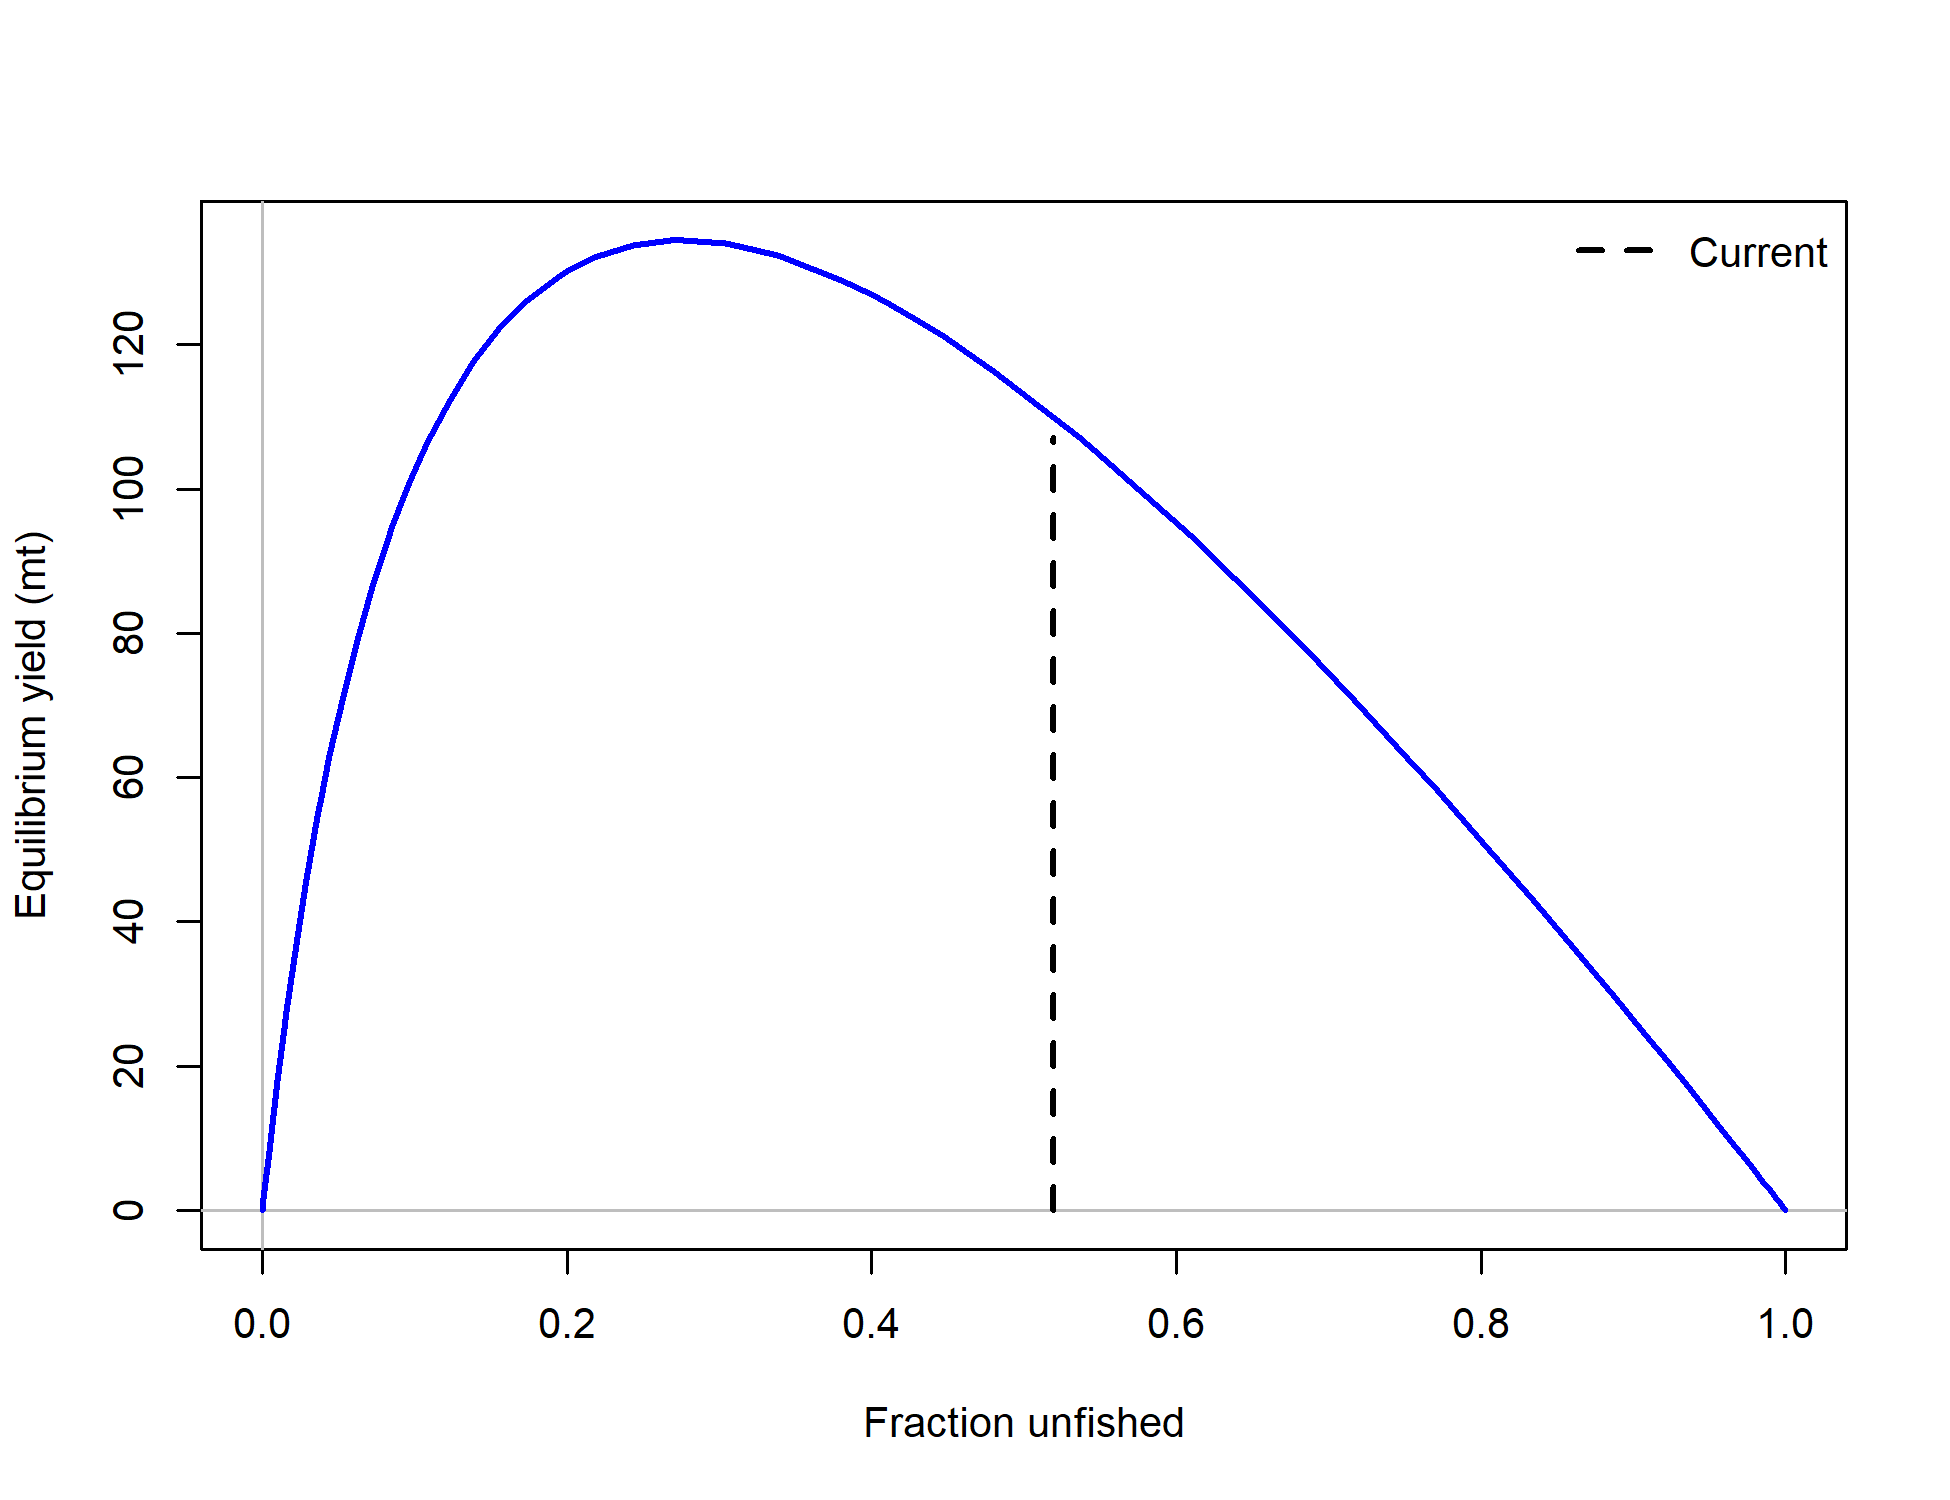
\includegraphics[width=1\textwidth,height=1\textheight]{N:/Assessments/CurrentAssessments/copper_rockfish_2023/models/nca/_bridging/2.4_dw/plots/yield2_yield_curve_with_refpoints.png}
\caption{Equilibrium yield curve for the base case model. Values are based on the 2020 fishery selectivities and with steepness fixed at 0.80.\label{fig:es-yield}}
\end{figure}

\hypertarget{management-performance}{%
\subsection*{Management performance}\label{management-performance}}
\addcontentsline{toc}{subsection}{Management performance}

Include Table of most recent 10 years of catches in comparison with OFL, ABC, HG, and OY/ACL values, overfishing levels, actual catch and discard. Include OFL (encountered), OFL (retained), and OFL (dead) if different due to discard and discard mortality.

\hypertarget{unresolved-problems-and-major-uncertainties}{%
\subsection*{Unresolved problems and major uncertainties}\label{unresolved-problems-and-major-uncertainties}}
\addcontentsline{toc}{subsection}{Unresolved problems and major uncertainties}

shared text

\hypertarget{decision-table-and-projections}{%
\subsection*{Decision table and projections}\label{decision-table-and-projections}}
\addcontentsline{toc}{subsection}{Decision table and projections}

Replace text with projected yields (OFL, ABC, and ACL), spawning biomass, and stock depletion levels for each year. OFL calculations should be based on the assumption that future catches equal ABCs and not OFLs.

\hypertarget{scientific-uncertainty}{%
\subsection*{Scientific uncertainty}\label{scientific-uncertainty}}
\addcontentsline{toc}{subsection}{Scientific uncertainty}

The model estimated uncertainty around the 2023 spawning output was \(\sigma\) = 0.32 and the uncertainty around the OFL was \(\sigma\) = 0.31. This is likely an underestimate of overall uncertainty because of the necessity to fix several population dynamic parameters (e.g., steepness, recruitment variance, female natural mortality) and no explicit incorporation of model structural uncertainty (although see the decision table for alternative states of nature).

\hypertarget{research-and-data-needs}{%
\subsection*{Research and data needs}\label{research-and-data-needs}}
\addcontentsline{toc}{subsection}{Research and data needs}

shared text

\pagebreak
\setlength{\parskip}{5mm plus1mm minus1mm}
\pagenumbering{arabic}
\setcounter{page}{1}
\renewcommand{\thefigure}{\arabic{figure}}
\renewcommand{\thetable}{\arabic{table}}
\setcounter{table}{0}
\setcounter{figure}{0}

\hypertarget{introduction}{%
\section{Introduction}\label{introduction}}

\hypertarget{basic-information}{%
\subsection{Basic Information}\label{basic-information}}

This assessment reports the status of copper rockfish (\emph{Sebastes caurinus}) off the California coast, north of Point Conception, using data through 2022.

Copper rockfish is a medium- to large-sized nearshore rockfish found from Mexico to Alaska. The core range is comparatively large, from northern Baja Mexico to the Gulf of Alaska, as well as in Puget Sound. Copper rockfish have historically been a part of both commercial and recreational fisheries throughout its range.

Copper rockfish are commonly found in waters less than 130 meters in depth in nearshore kelp forests and rocky habitat (Love 1996). The diets of copper rockfish consist primarily of crustaceans, mollusks, and fish (Lea, McAllister, and VenTresca 1999; Bizzarro, Yoklavich, and Wakefield 2017). The body coloring of copper rockfish varies across the West Coast with northern fish often exhibiting dark brown to olive with southern fish exhibiting yellow to olive-pink variations in color (D. J. Miller and Lea 1972), which initially led to them being designated as two separate species (\emph{S. caurinus} and \emph{S. vexillaris}).

Numerous genetic studies have been performed looking for genetic variation in copper rockfish, with variable outcomes. Genetic work has revealed significant differences between Puget Sound and coastal stocks (S. Dick, Shurin, and Taylor 2014). Stocks along the West Coast have not been determined to be genetically distinct populations, but significant population subdivision has been detected, indicating limited oceanographic exchange among geographically proximate locations (Buonaccorsi et al. 2002; Johansson et al. 2008). A specific study examining copper rockfish populations off the coast of Santa Barbara and Monterey California identified a genetic break between the north and south, with moderate differentiation (Sivasundar and Palumbi 2010).

Copper rockfish are a relatively long-lived rockfish, estimated to live at least 50 years (Love 1996). Copper rockfish was determined to have the highest vulnerability (V = 2.27) of any West Coast groundfish stock evaluated in a productivity susceptibility analysis (J. M. Cope et al. 2011). This analysis calculated species-specific vulnerability scores based on two dimensions: productivity characterized by the life history and susceptibility that characterized how the stock could be impacted by fisheries and other activities.

\hypertarget{life-history}{%
\subsection{Life History}\label{life-history}}

Replace text.

\hypertarget{ecosystem-considerations-1}{%
\subsection{Ecosystem Considerations}\label{ecosystem-considerations-1}}

Replace text.

\hypertarget{historical-and-current-fishery-information}{%
\subsection{Historical and Current Fishery Information}\label{historical-and-current-fishery-information}}

Off the coast of California, north of Point Conception, copper rockfish is caught in both commercial and recreational fisheries. Recreational removals have been the largest source of fishing mortality, comprising nearly 85 percent of total removals of copper rockfish across all years (Table XX and Figure XX). The landings from the commercial fishery have been minimal by year, expect for a brief period between the mid-1980s and early-2000s.

The recreational fishery in the early part of the 20th century was focused on nearshore waters near ports, with expanded activity further from port and into deeper depths over time (R. R. Miller et al. 2014). Prior to the groundfish fishery being declared a federal disaster in 2000, and the subsequent rebuilding period, there were no time or area closures for groundfish. Access to deeper depths during this period spread effort over a larger area and filled bag limits with a greater diversity of species from both the shelf and nearshore. This resulted in lower catch of nearshore rockfish relative to the period after 2000 when 20 to 60 fm depth restrictions ranging from 20 fm in the Northern Management Area to 60 fm in the Southern Management Area were put in place in various management area delineations along the state (see Appendix Section \ref{ca-man}). This shifting effort onto the nearshore, concomitantly increased catch rates for nearshore rockfish including copper rockfish in the remaining open depths, though season lengths were greatly curtailed.

Following all previously overfished groundfish species, other than yelloweye rockfish, being declared rebuilt by 2019, deeper depth restrictions were offered in the Southern Management area allowing resumed access to shelf rockfish in less than 75 fm and are currently 100 fm as of 2021. The increased access to deeper depths south of Point Conception with the rebuilding of cowcod is expected to reduce the effort in nearshore waters where copper rockfish is most prevalent. To the north of Point Conception where yelloweye rockfish are prevalent, depth constraints persist and effort remains focused on the nearshore in 30 to 50 fm depending on the management area. As yelloweye rockfish continues to rebuild, incremental increases in access to deeper depths are expected, which will likely further reduce the effort in nearshore waters where copper rockfish is most prevalent.

Prior to development of the live fish market in the 1980s, there was very little commercial catch of copper rockfish, with dead copper rockfish fetching a low ex-vessel price per pound. Copper rockfish were targeted along with other rockfish to some degree in the nearshore or caught as incidental catch by vessels targeting other more valuable stocks such as lingcod. Most fish were caught using hook and line gear, though some were caught using traps, gill nets and, rarely, trawl gear. Trawling was prohibited within three miles of shore in 1953 and gill netting within three miles of shore was prohibited in 1994, preventing access to a high proportion of the species habitat with these gear types. Copper rockfish were caught along with other rockfish to some degree in the nearshore or caught as bycatch by vessels targeting other more valuable stocks such as lingcod.

In the late 1980s and early 1990s a market for fish landed live arose out of Los Angeles and the Bay area, driven by demand from Asian restaurants and markets. The growth of the live fish market was driven by consumers willing to pay a higher price for live fish, ideally plate-sized (12 - 14 inches or 30.5 - 35.6 cm). Live fish landed for the restaurant market are lumped into two categories, small (1 - 3 lbs.) or large (3 - 6 lbs.), with small, plate-sized, fish fetching higher prices at market ranging between \$5 -7 per fish (Bill James, personal communication). Copper rockfish is one of the many rockfish species that is included in the commercial live fish fishery. The proportion of copper rockfish being landed live vs.~dead since 2000 by California commercial fleets ranges between 50 to greater than 70 percent in the southern and northern areas, respectively.

With the development and expansion of the nearshore live fish fishery during the 1980s and 1990s, new entrants in this open access fishery were drawn by premium ex-vessel price per pound for live fish, resulting in over-capitalization of the fishery. Since 2002, the California Department of Fish and Wildlife (CDFW) has managed 19 nearshore species in accordance with Nearshore Fisheries Management Plan (Wilson-Vandenberg, Larinto, and Key 2014). In 2003, the CDFW implemented a Nearshore Restricted Access Permit system, including the requirement of a Deeper Nearshore Fishery Species Permit to retain copper rockfish, with the overall goal of reducing the number of participants to a more sustainable level, with permit issuance based on historical landings history by the retrospective qualifying date. The result was a reduction in permits issued from 1,127 in 1999 to 505 in 2003, greatly reducing catch levels. In addition, reduced trip limits, season closures in March and April and depth restrictions were implemented to address bycatch of overfished species and associated constraints from their low catch limits.

Copper rockfish residing between Point Conception and the California/Oregon border are assessed here as a single, separate stock (Figure \ref{fig:map}). This designation was made based on oceanographic, geographic, and fishery conditions. The copper rockfish population in California waters was split at Point Conception due to water circulation patterns that create a natural barrier between nearshore rockfish populations to the north and south. The northern border for this assessment was defined as the California/Oregon border due to substantial differences in historical and current exploitation levels. Additionally, the fairly sedentary nature of adult copper rockfish, likely limits flow of fish between northern California and areas to the north.

\hypertarget{summary-of-management-history-and-performance}{%
\subsection{Summary of Management History and Performance}\label{summary-of-management-history-and-performance}}

Replace text.

\hypertarget{foreign-fisheries}{%
\subsection{Foreign Fisheries}\label{foreign-fisheries}}

Replace text.

\hypertarget{data}{%
\section{Data}\label{data}}

Data comprise the foundational components of stock assessment models. The decision to include or exclude particular data sources in an assessment model depends on many factors. These factors often include, but are not limited to, the way in which data were collected (e.g., measurement method and consistency); the spatial and temporal coverage of the data; the quantity of data available per desired sampling unit; the representativeness of the data to inform the modeled processes of importance; timing of when the data were provided; limitations imposed by the Terms of Reference; and the presence of an avenue for the inclusion of the data in the assessment model. Attributes associated with a data source can change through time, as can the applicability of the data source when different modeling approaches are explored (e.g., stock structure or time-varying processes). Therefore, the specific data sources included or excluded from this assessment should not necessarily constrain the selection of data sources applicable to future stock assessments for copper rockfish. Even if a data source is not directly used in the stock assessment they can provide valuable insights into biology, fishery behavior, or localized dynamics.

Data from a wide range of programs were available for possible inclusion in the current assessment model. Descriptions of each data source included in the model (Figure \ref{fig:data-plot}) and sources that were explored but not included in the base model are provided below. Data that were excluded from the base model were explicitly explored during the development of this stock assessment or have not changed since their past exploration in a previous copper rockfish stock assessment. In some cases, the inclusion of excluded data sources were explored through sensitivity analyses (see Section \ref{assessment-model}).

\hypertarget{fishery-dependent-data}{%
\subsection{Fishery-Dependent Data}\label{fishery-dependent-data}}

\hypertarget{commercial-fishery}{%
\subsubsection{Commercial Fishery}\label{commercial-fishery}}

\hfill\break

Commercial landings prior to 1969 were extracted from the Southwest Fisheries Science Center (SWFSC) landings reconstruction database for estimates from the California Catch Reconstruction (Ralston et al. 2010). Landings in this database are divided into trawl, non-trawl, and unknown gear categories. Regions 7 and 8 as defined by Ralston et al. (2010) were assigned to south of Point Conception in California. Regions 2, 4, and 5 are associated with areas north of Point Conception. Region 6 in Ralston et al. (2010) included Santa Barbara County (mainly south of Point Conception), plus some major ports north of Point Conception. To allocate landings from Region 6 to the areas north and south of Point Conception, we followed an approach used by Dick et al. (2007) for the assessment of cowcod. Specifically, port-specific landings of total rockfish from the CDFW Fish Bulletin series were used to determine the annual fraction of landings in Region 6 that was north and south of Point Conception (Table \ref{tab:com-ratio}). Rockfish landings at that time were not reported at the species level. Although the use of total rockfish landings to partition landings in Region 6 is not ideal, we see this as the best available option in the absence of port-specific species composition data. Landings from unknown locations (Region 0) were allocated proportional to the landings from known regions.

In September 2005, the California Cooperative Groundfish Survey (CCGS) incorporated newly acquired commercial landings statistics from 1969-1980 into the CALCOM database (Pearson, Erwin, and Key 2008). The data consisted of landing receipts (``fish tickets''), including mixed species categories for rockfish. In order to assign rockfish landings to individual species, the earliest available species composition samples were applied to the fish ticket data by port, gear, and quarter. These `ratio estimator' landings are coded (internally) as market category 977 in the CALCOM database, and are used in this and past assessments as the best available landings for the time period 1969-1980 for all port complexes. See Appendix A of Dick et al. (2007) for further details.

Commercial fishery landings from 1981-2022 were extracted from the Pacific Fisheries Information Network (PacFIN) database (extracted February 6, 2023). Landings were separated north and south of Point Conception based on port of landing. Commercial landings for copper rockfish were split into two fleets based on the fish landed condition, live or dead, and aggregated across gear types (Table \ref{tab:allcatches} and Figure \ref{fig:catch}). The selection of this fleet structure was based on potential differences in selectivity by the fishery based on fish landed condition where the live fish fishery may be targeting fish of particular sizes (i.e., plate sized). The first year where fish were observed to be landed live for copper rockfish in the area south of Point Conception was 1994.

Discarding was not estimated within the model. The commercial catches, landings plus discards, were estimated external to the model based on data from the West Coast Groundfish Observer Program (WCGOP) data provided in the Groundfish Expanded Mortality Multiyear (GEMM) product. The GEMM provides expanded estimates of landings, discard, and catches based on observed trips by sector split north and south of 40\(^\circ\) 10' N. lat. for the commercial fishery. Estimated landings and discards south of 40\(^\circ\) 10' N. lat. from select sectors (LE Fixed Gear DTL - Hook and Line, Nearshore, CS - Hook and Line, OA Fixed Gear - Hook and Line, OA Fixed Gear - Pot, and LE Fixed Gear DTL - Pot) were used to calculate a discard rate (total discard divided by the sum of landings and discards by year) for 2002-2021. The annual discard rates were applied to the total landings by year to calculate catches for both areas south and north of Point Conception. The median discard rate south of 40\(^\circ\) 10' N. lat. from the select sectors between 2002-2021 in the GEMM was 3 percent. This discard rate was applied to landings between 1916-2001 and 2022 to determine catch by year. The assumptions around the discard rate by year had limited impact to the assumed total catches given the limited scale of removals by the commercial fishery for copper rockfish. Across all years, 1916-2022, the landings were increased by 2-3 percent by area (11 mt south of Point Conception and 26 mt north of Point Conception) to calculate the total catches.

\hypertarget{landings-and-discards}{%
\paragraph{Landings and Discards}\label{landings-and-discards}}

\hypertarget{composition-data}{%
\paragraph{Composition Data}\label{composition-data}}

\hypertarget{recreational-fishery}{%
\subsubsection{Recreational Fishery}\label{recreational-fishery}}

\hypertarget{landings-and-discards-1}{%
\paragraph{Landings and Discards}\label{landings-and-discards-1}}

\hfill\break

The recreational fishery is the main source of exploitation of copper rockfish across California. The recreational catches of copper rockfish south of Point Conception in California waters peaked in the late 1970s and early 1980s. Catches declined in the 1990s and early 2000s (Table \ref{tab:allcatches} and Figure \ref{fig:catch}). The removals remained relatively low until 2015. Catches begun to increase in 2015, likely due to changes in harvest specifications (J. Cope et al. 2013). The catches decreased in 2020 due to COVID-19 impacts and remained relatively low in 2021 and 2022 due to reductions in the sub-bag limits in California for copper rockfish. The recreational fishery was split into two fleets based on fishing type (termed `modes'), a commercial passenger fishing vessel (CPFV, party/charter mode) fleet and a combined private or rental boats (PR mode) and shoreside (man-made and beach/bank modes) fleet. The catches associated with the shoreside mode for copper rockfish are limited and did not justify a separate fishing fleet within the model.

Recreational landing estimates from 1928 to 1980 were obtained from the historical reconstruction (Ralston et al. 2010). The historical landings reconstruction split removals north and south of Point Conception and by recreational modes. CPFV landings of all rockfish were based on logbook data (which do not report rockfish to the species level), scaled by compliance estimates, while total recreational landings from PR vessels were based on a combination of the relative catch rates observed in the CPFV fleet and a linear ramp between catch estimates in the early 1960s and those in the early 1980s (as described in Ralston et al. (2010)). The species composition of rockfish landings was estimated using a combination of the 1980s Marine Recreational Fisheries Statistics Survey (MRFSS) data as well as limited CPFV mode species composition data from onboard observer programs in the late 1970s (south of Point Conception) and dockside recreational creel surveys in the late 1950s and early 1960s (north of Point Conception).

Recreational removals from 1981-1989 and 1993-2003 were obtained from MRFSS downloaded from the Recreational Fisheries Information Network (RecFIN). Historically, copper rockfish were occasionally referred to as whitebelly rockfish in select California areas. MRFSS catches were pulled for both species names and for all ocean areas. MRFSS includes estimates of removals for 1980. However, due to inconsistencies in the estimates of this year in MRFSS, likely due to it being the first year of the survey with low sample sizes, the value for recreational landings from the historical reconstruction were used (2010).

Some known issues with the MRFSS estimates include 1) a change in the spatial definition of California subregions after 1989, 2) missing or imprecise estimates of catch in weight for some strata that reported catch in numbers, and 3) a hiatus in sampling from 1990-1992 (all modes) and also 1993-1995 in the party/charter mode north of Point Conception. The STAT attempted to address each of these issues, as described below. CRFS estimates from 2004 were also included in the MRFSS analysis, as they were not available on the current RecFIN website but are included with the MRFSS catch estimate tables

The MRFSS definition of ``Southern California'' included San Luis Obispo County between 1981-1989, requiring the catches from this county to be split out and removed from the recreational catch south of Point Conception. The MRFSS catches between southern and northern California were adjusted in a similar fashion as previous assessments split at Point Conception. Albin et al. (1993) used MRFSS data to estimate catch at a finer spatial scale from the California/Oregon border to the southern edge of San Luis Obispo (SLO) County. Over the period 1981-1986, numbers of copper rockfish landed in SLO County were found to be approximately one third (0.317) of the numbers of copper rockfish landed in all California counties north of SLO County (Albin, Karpov, and Van Buskirk 1993). Therefore, to approximate catches north and south of Point Conception from 1980-1989, the STAT reduced the `southern' subregion annual catch (which included SLO County) from 1980-1989 by 0.317 during the same period, and added this amount to the northern subregion catch. On average, this `moves' the estimated SLO County catch from the southern region to the northern region from 1980-1989, creating a spatially consistent time series of landings over the entire time series.

The STAT chose to use catch in terms of weight (WGT\_AB1 column) within MRFSS. The catch weights were converted from kilograms to metric tons and any records with missing catch weights were examined. The number of records with missing catch weights for copper rockfish in MRFSS were limited (only 18 out of 713). The missing catch weights were imputed based on the number of fish (TOT\_CAT column) and the calculated average fish weight by year and area north and south of Point Conception.

MRFSS sampling was halted from 1990-1992 due to funding issues. The survey resumed in 1993 in all modes, except for the PC boat mode which resumed in 1996 for counties north of Santa Barbara County. To produce catch estimates for the missing subregion, mode, and year combinations linear interpolations were used to fill in the missing data.

Two additional revisions were applied to select years and modes in the MRFSS data based on conversations with California Department of Fish and Wildlife (CDFW). The catches for the PR mode north of Point Conception in MRFSS for 1981 were 50 to 90 percent greater than the catches in 1980 and 1982, respectively. The high catches in this year were assumed to be a result of issues in the catch expansions due to limited sampling. The catches for the PR fleet were revised downward to be equal to the average removals in surrounding years (1979, 1980, 1982, and 1983). The catches in MRFSS south of Point Conception in 1987 were identified as abnormally low by CDFW (John Budrick, pers. communication, 13 to 27 percent of catches in 1986 and 1988) which was due to no catch information for waves 1-3 (January - June) for either mode. Absence of data in 1987 for these waves was not observed across other rockfish species in southern California indicating that the absence of catch data was likely not due to closures in the fishery. The catches for this year and mode were set equal to the average catch by mode 2 years before and after 1987.

Recreational landings from 2004-2022 were obtained from California Recreational Fisheries Survey (CRFS) available on RecFIN for for all ocean areas. This survey improves upon the MRFSS sampling design, employing higher sampling rates and producing estimates with finer spatial and temporal resolution. CRFS also employs onboard CPFV observers, providing spatially referenced, drift-level estimates of catch and discard for a subset of anglers on observed groundfish trips. Any CRFS records of fish caught in Mexican waters were removed and catch estimates were split north and south of Point Conception for each fleet. Due to database issues, catches for 2004 are currently not available on RecFIN. The catches for this year were set equal to data pulled in 2021 for the previous assessment of copper rockfish.

Adjustments to the recreational catches for 2020-2022 were provided directly by CDFW to deal with sampling issues due to COVID-19. During 2020 dockside sampling by observers was halted April through June leading to missing catch data within the CRFS database for this period. CDFW provided proxy catch values for these months directly by CRFS district (personal communication, Melanie Parker). The total proxy catches south of Point Conception (districts 1 and 2) for these months were 18.9 mt and 15.0 mt north of Point Conception in California (districts 3 - 6). These catches were split by mode (CPFV and PR) equally for both areas, noting that effort by mode during this period varied across district based on varying COVID-19 restrictions. When sampling resumed a large number of rockfish catches were not identified to species, recorded as rockfish genus, for the remainder of 2020 and 2021 due to social distancing for health and safety. The second adjustment to catches was to allocated unidentified rockfish catches. CDFW provided proxy catch values that allocated a subset of the rockfish genus removals by recreational mode north and south of Point Conception for these years. Finally, the completed catch estimates for 2022 were not available within CRFS on RecFIN by the data deadline for this assessment and estimates were provided directly to the STAT from CDFW.

MRFSS and CRFS both provide estimates of total mortality which combine observed landings plus estimates of discarded fish using depth-dependent mortality rates. While the recreational removals from the historical reconstruction from 1928-1980 account for only landed fish. There is limited information on historical discarding in the recreational fishery. A report by Miller and Gotshall (1965) looked at the number of retained and discard fish in the recreational fishery in California for a select year which showed essentially no discarding of copper rockfish. Based on that no additional discards were applied to the historical data between 1926-190.

\hypertarget{indices-of-abundance}{%
\paragraph{Indices of Abundance}\label{indices-of-abundance}}

\hfill\break

Appendix Section \ref{mrfs-index}

Appendix Section \ref{onboard-cpfv-index}

Appendix Section \ref{dwv-cpfv-index}

Appendix Section \ref{crfs-pr-index}

\hypertarget{composition-data-1}{%
\paragraph{Composition Data}\label{composition-data-1}}

\hypertarget{fishery-independent-data}{%
\subsection{Fishery-Independent Data}\label{fishery-independent-data}}

\hypertarget{california-cooperative-fisheries-research-program-survey}{%
\subsubsection{California Cooperative Fisheries Research Program Survey}\label{california-cooperative-fisheries-research-program-survey}}

\hypertarget{index-of-abundance}{%
\paragraph{Index of Abundance}\label{index-of-abundance}}

\hfill\break

Since 2007, the \gls{s-ccfrp} has monitored several areas in California to evaluate the performance of \glspl{mpa} and understand nearshore fish populations (Wendt and Starr 2009; Starr et al. 2015). In 2017, the survey expanded beyond the four \Gls{mpa}s in central California (Año Nuevo, Point Lobos, Point Buchon, and Piedras Blancas) to include the entire California coast. Fish are collected by volunteer anglers aboard \glspl{cpfv} guided by one of the following academic institutions based on proximity to fishing location: Humboldt State University; Bodega Marine Laboratories; Moss Landing Marine Laboratories; Cal Poly San Luis Obispo; University of California, Santa Barbara; and Scripps Institution of Oceanography.

Surveys consist of fishing with hook-and-line gear for 30-45 minutes within randomly chosen 500 by 500 m grid cells within and outside \glspl{mpa}. Prior to 2017, all fish were measured for length and release or descended to depth; since then, some were sampled for otoliths and fin clips.

Appendix Section \ref{#ccfrp-index}

\hypertarget{composition-data-2}{%
\paragraph{Composition Data}\label{composition-data-2}}

\hypertarget{california-department-of-fish-and-wildlife-remotely-operated-vehicle-survey}{%
\subsubsection{California Department of Fish and Wildlife Remotely Operated Vehicle Survey}\label{california-department-of-fish-and-wildlife-remotely-operated-vehicle-survey}}

\hypertarget{index-of-abundance-1}{%
\paragraph{Index of Abundance}\label{index-of-abundance-1}}

\hfill\break

The California Department of Fish and Wildlife (CDFW) in collaboration with Marine Applied Research and Exploration (MARE) have been conducting remotely operated vehicle (ROV) surveys along the California coast in Marine Protected Areas (MPAs) and reference sites adjacent to them since 2004 for the purposes of long-term monitoring of changes in size, density (fish/square meter) and length of fish and invertebrate species along the California coast. Surveys of the entire coast have now been undertaken twice, each taking three years to complete, 2014-2016 and again in 2019-2021. The survey conducted multiple 500 meter transects across rocky reef survey sites. Sample sites were selected by first randomly selecting the deepest transect at a given site, then selecting transects on a constant interval into shallower depths. Transects were designed to be oriented parallel to general depth contours, though they were carried out using a fixed bearing that crossed depths in some cases.

The data were explored using a super year approach where the central years, 2015 and 2020, were designated as the super year and the data were split north and south of Point Conception. The effort of the survey were split roughly equally between sites that were within MPAs or areas open to fishing (referred to as ``Reference'') with sampling across most sites (termed ``MPA group'') within each super year. The number of transects and the number of copper rockfish by site and super year are shown in Table \ref{tab:rov-obs}.

Figure \ref{fig:rov-obs-loc}

he trend in the calculated catch-per-unit-effort based on the data alone was highly variable across sampling locations and by MPA or Reference area (Figure \ref{fig:rov-raw-cpue}).

CDFW provided an initial analysis of the CDFW ROV survey data which helped form the considered modeling approaches for these data.

The STAT explored alternative model structures to generate a standardized index of relative abundance for this survey. The final model selected was a model

Details regarding the index of abundance, sample sizes and model selection can be found in the Appendix Section \ref{cdfw-rov-index}.

\hypertarget{composition-data-3}{%
\paragraph{Composition Data}\label{composition-data-3}}

\hfill\break

Length measurement were made from images taken with stereo-cameras by the CDFW ROV survey in 2016, 2019, 2020, and 2021.

Figure \ref{fig:rov-len}

\hypertarget{northwest-fisheries-science-center-west-coast-groundfish-bottom-trawl-survey}{%
\subsubsection{Northwest Fisheries Science Center West Coast Groundfish Bottom Trawl Survey}\label{northwest-fisheries-science-center-west-coast-groundfish-bottom-trawl-survey}}

\hfill\break

The \Gls{s-wcgbt} is based on a random-grid design; covering the coastal waters from a depth of 55-1,280 m (Bradburn, Keller, and Horness 2011). This design generally uses four industry-chartered vessels per year assigned to a roughly equal number of randomly selected grid cells and divided into two `passes' of the coast. Two vessels fish from north to south during each pass between late May to early October. This design therefore incorporates both vessel-to-vessel differences in catchability, as well as variance associated with selecting a relatively small number (approximately 700) of possible cells from a very large set of possible cells spread from the Mexican to the Canadian borders.

\hypertarget{biological-data}{%
\subsection{Biological Data}\label{biological-data}}

\hypertarget{natural-mortality}{%
\subsubsection{Natural Mortality}\label{natural-mortality}}

\hfill\break

Natural mortality was not directly measured, so life-history based empirical relationships were used. The Natural Mortality Tool (NMT), a Shiny-based graphical user interface allowing for the application of a variety of natural mortality estimators based on measures such as longevity, size, age and growth, and maturity, was used to obtain estimates of natural mortality. The NMT currently provides 19 options, including the Hamel (\textbf{hamel\_development\_2022?}) method, which is a corrected form of the Then et al. (2015) functional regression model and is a commonly applied method for West Coast groundfish. The NMT also allows for the construction of a natural mortality prior weighted across methods by the user.

The Hamel (\textbf{hamel\_development\_2022?}) method for developing a prior on natural mortality for West Coast groundfish stock assessments combines meta-analytic approaches relating the \(M\) rate to other life-history parameters such as longevity, size, growth rate, and reproductive effort to provide a prior for \(M\). The Hamel (\textbf{hamel\_development\_2022?}) method re-evaluated the data used by Then et al. (2015) by fitting the one-parameter \(A_{\text{max}}\) model under a log-log transformation (such that the slope is forced to be -1 in the transformed space (Hamel 2015), the point estimate and median of the prior for \(M\) is:

\begin{centering}

$M=\frac{5.4}{A_{\text{max}}}$

\end{centering}

\vspace{0.5cm}

where \(A_{\text{max}}\) is the maximum age. The prior is defined as a lognormal distribution with mean \(ln(5.4/A_{\text{max}})\) and standard error = 0.31. Using a maximum age of 50, the point estimate and median of the prior is 0.108 yr\textsuperscript{-1}. The maximum age was selected based on available age data from all West Coast data sources and literature values. The oldest aged copper rockfish was 51 years with two observations, one each off of the coast of Washington and Oregon in 2019.

ADD INFORMATION ABOUT THE OLDEST OBSERVATION IN CALIFORNIA.

The maximum age in the model was set at 50 years. This selection was consistent with the literature examining the longevity of copper rockfish within California (Love 1996) and was supported by the observed ages that had multiple observations of fish between 44 and 51 years of age.

\hypertarget{maturation-and-fecundity}{%
\subsubsection{Maturation and Fecundity}\label{maturation-and-fecundity}}

\hypertarget{sex-ratio}{%
\subsubsection{Sex Ratio}\label{sex-ratio}}

\hfill\break

There were limited sex-specific observations by length or age across biological data sources. The sex ratio of copper rockfish by length and age across all available data sources off the West Coast are shown in Figure \ref{fig:frac-sex-len}. The sex ratio of young fish was assumed to be 1:1.

\hypertarget{length-weight-relationship}{%
\subsubsection{Length-Weight Relationship}\label{length-weight-relationship}}

\hfill\break

The length-weight relationship for copper rockfish was estimated outside the model using all coastwide biological data available from fishery-independent data from the \gls{s-wcgbt} and the NWFSC Hook and Line survey. The estimated length-weight relationship for female fish was W = 9.56e-06\(L\)\textsuperscript{3.19} and males 1.08e-05\(L\)\textsuperscript{3.15} where \(L\) is length in cm and W is weight in kilograms (Figure \ref{fig:weight-length}).

\hypertarget{growth-length-at-age}{%
\subsubsection{Growth (Length-at-Age)}\label{growth-length-at-age}}

\hypertarget{ageing-precision-and-bias}{%
\subsubsection{Ageing Precision and Bias}\label{ageing-precision-and-bias}}

\hypertarget{environmental-and-ecosystem-data}{%
\subsection{Environmental and Ecosystem Data}\label{environmental-and-ecosystem-data}}

\hypertarget{assessment-model}{%
\section{Assessment Model}\label{assessment-model}}

\hypertarget{summary-of-previous-assessments-and-reviews}{%
\subsection{Summary of Previous Assessments and Reviews}\label{summary-of-previous-assessments-and-reviews}}

\hypertarget{history-of-modeling-approaches-not-required-for-an-update-assessment}{%
\subsubsection{History of Modeling Approaches (not required for an update assessment)}\label{history-of-modeling-approaches-not-required-for-an-update-assessment}}

\hypertarget{most-recent-star-panel-and-ssc-recommendations-not-required-for-an-update-assessment}{%
\subsubsection{Most Recent STAR Panel and SSC Recommendations (not required for an update assessment)}\label{most-recent-star-panel-and-ssc-recommendations-not-required-for-an-update-assessment}}

\hypertarget{response-to-groundfish-subcommittee-requests-not-required-in-draft}{%
\subsubsection{Response to Groundfish Subcommittee Requests (not required in draft)}\label{response-to-groundfish-subcommittee-requests-not-required-in-draft}}

\hypertarget{model-structure-and-assumptions}{%
\subsection{Model Structure and Assumptions}\label{model-structure-and-assumptions}}

\hypertarget{model-changes-from-the-last-assessment-not-required-for-an-update-assessment}{%
\subsubsection{Model Changes from the Last Assessment (not required for an update assessment)}\label{model-changes-from-the-last-assessment-not-required-for-an-update-assessment}}

\hypertarget{modeling-platform-and-structure}{%
\subsubsection{Modeling Platform and Structure}\label{modeling-platform-and-structure}}

General model specifications (e.g., executable version, model structure, definition of fleets and areas)

\hypertarget{model-parameters}{%
\subsubsection{Model Parameters}\label{model-parameters}}

Describe estimated vs.~fixed parameters, priors

\hypertarget{key-assumptions-and-structural-choices}{%
\subsubsection{Key Assumptions and Structural Choices}\label{key-assumptions-and-structural-choices}}

\hypertarget{base-model-results}{%
\subsection{Base Model Results}\label{base-model-results}}

\hypertarget{parameter-estimates}{%
\subsubsection{Parameter Estimates}\label{parameter-estimates}}

\hypertarget{fits-to-the-data}{%
\subsubsection{Fits to the Data}\label{fits-to-the-data}}

\hypertarget{population-trajectory}{%
\subsubsection{Population Trajectory}\label{population-trajectory}}

\hypertarget{reference-points-1}{%
\subsubsection{Reference Points}\label{reference-points-1}}

\hypertarget{model-diagnostics}{%
\subsection{Model Diagnostics}\label{model-diagnostics}}

Describe all diagnostics

\hypertarget{convergence}{%
\subsubsection{Convergence}\label{convergence}}

\hypertarget{sensitivity-analyses}{%
\subsubsection{Sensitivity Analyses}\label{sensitivity-analyses}}

\hypertarget{retrospective-analysis}{%
\subsubsection{Retrospective Analysis}\label{retrospective-analysis}}

\hypertarget{likelihood-profiles}{%
\subsubsection{Likelihood Profiles}\label{likelihood-profiles}}

\hypertarget{unresolved-problems-and-major-uncertainties-1}{%
\subsubsection{Unresolved Problems and Major Uncertainties}\label{unresolved-problems-and-major-uncertainties-1}}

\hypertarget{management}{%
\section{Management}\label{management}}

\hypertarget{reference-points-2}{%
\subsection{Reference Points}\label{reference-points-2}}

\hypertarget{unresolved-problems-and-major-uncertainties-2}{%
\subsection{Unresolved Problems and Major Uncertainties}\label{unresolved-problems-and-major-uncertainties-2}}

\hypertarget{harvest-projections-and-decision-tables}{%
\subsection{Harvest Projections and Decision Tables}\label{harvest-projections-and-decision-tables}}

\hypertarget{evaluation-of-scientific-uncertainty}{%
\subsection{Evaluation of Scientific Uncertainty}\label{evaluation-of-scientific-uncertainty}}

\hypertarget{research-and-data-needs-1}{%
\subsection{Research and Data Needs}\label{research-and-data-needs-1}}

\hypertarget{acknowledgments}{%
\section{Acknowledgments}\label{acknowledgments}}

Here are all the mad props!

\clearpage

\hypertarget{references}{%
\section{References}\label{references}}

\hypertarget{refs}{}
\begin{CSLReferences}{1}{0}
\leavevmode\vadjust pre{\hypertarget{ref-albin_effort_1993}{}}%
Albin, Douglas P, Konstantin A Karpov, and Wade H. Van Buskirk. 1993. {``Effort and Catch Estimates for {Northern} and {Central} {California} Marine Recreational Fisheries, 1981-1986.''} Administrative Report No. 93-3. State of California The Resources Agency Department of Fish; Game.

\leavevmode\vadjust pre{\hypertarget{ref-bizzarro_diet_2017-1}{}}%
Bizzarro, Joseph J., Mary M. Yoklavich, and W. Waldo Wakefield. 2017. {``Diet Composition and Foraging Ecology of {U}.{S}. {Pacific} {Coast} Groundfishes with Applications for Fisheries Management.''} \emph{Environmental Biology of Fishes} 100 (4): 375--93. \url{https://doi.org/10.1007/s10641-016-0529-2}.

\leavevmode\vadjust pre{\hypertarget{ref-bradburn_2003_2011}{}}%
Bradburn, M. J., A. A Keller, and B. H. Horness. 2011. {``The 2003 to 2008 {US} {West} {Coast} Bottom Trawl Surveys of Groundfish Resources Off {Washington}, {Oregon}, and {California}: Estimates of Distribution, Abundance, Length, and Age Composition.''} US Department of Commerce, National Oceanic; Atmospheric Administration, National Marine Fisheries Service.

\leavevmode\vadjust pre{\hypertarget{ref-buonaccorsi_population_2002}{}}%
Buonaccorsi, Vincent P, Carol A Kimbrell, Eric A Lynn, and Russell D Vetter. 2002. {``Population Structure of Copper Rockfish (\emph{{Sebastes} Caurinus}) Reflects Postglacial Colonization and Contemporary Patterns of Larval Dispersal.''} \emph{Canadian Journal of Fisheries and Aquatic Sciences} 59 (8): 1374--84. \url{https://doi.org/10.1139/f02-101}.

\leavevmode\vadjust pre{\hypertarget{ref-cope_approach_2011}{}}%
Cope, Jason M., John DeVore, E. J. Dick, Kelly Ames, John Budrick, Daniel L. Erickson, Joanna Grebel, et al. 2011. {``An {Approach} to {Defining} {Stock} {Complexes} for {U}.{S}. {West} {Coast} {Groundfishes} {Using} {Vulnerabilities} and {Ecological} {Distributions}.''} \emph{North American Journal of Fisheries Management} 31 (4): 589--604. \url{https://doi.org/10.1080/02755947.2011.591264}.

\leavevmode\vadjust pre{\hypertarget{ref-cope_data-moderate_2013}{}}%
Cope, Jason, E. J. Dick, Alec MacCall, Melissa Monk, Braden Soper, and Chantel Wetzel. 2013. {``Data-Moderate Stock Assessments for Brown, {China}, Copper, Sharpchin, Stripetail, and Yellowtail Rockfishes and {English} and Rex Soles in 2013.''} 7700 Ambassador Place NE, Suite 200, Portland, OR: Pacific Fishery Management Council. \url{http://www.academia.edu/download/44999856/CopeetalDataModerate2013.pdf}.

\leavevmode\vadjust pre{\hypertarget{ref-dick_status_2007}{}}%
Dick, E. J., Stephen Ralston, and Don E. Pearson. 2007. {``Status of Cowcod, \emph{{Sebastes} Levis}, in the {Southern} {California} {Bight}.''} Pacific Fishery Management Council, 7700 Ambassador Place NE, Suite 200, Portland, OR 97220.

\leavevmode\vadjust pre{\hypertarget{ref-dick_replicate_2014}{}}%
Dick, S., J. B. Shurin, and E. B. Taylor. 2014. {``Replicate Divergence Between and Within Sounds in a Marine Fish: The Copper Rockfish ( \emph{{Sebastes} Caurinus} ).''} \emph{Molecular Ecology} 23 (3): 575--90. \url{https://doi.org/10.1111/mec.12630}.

\leavevmode\vadjust pre{\hypertarget{ref-hamel_method_2015}{}}%
Hamel, Owen S. 2015. {``A Method for Calculating a Meta-Analytical Prior for the Natural Mortality Rate Using Multiple Life History Correlates.''} \emph{ICES Journal of Marine Science: Journal Du Conseil} 72 (1): 62--69. \url{https://doi.org/10.1093/icesjms/fsu131}.

\leavevmode\vadjust pre{\hypertarget{ref-johansson_influence_2008}{}}%
Johansson, M. L., M. A. Banks, K. D. Glunt, H. M. Hassel-Finnegan, and V. P. Buonaccorsi. 2008. {``Influence of Habitat Discontinuity, Geographical Distance, and Oceanography on Fine-Scale Population Genetic Structure of Copper Rockfish ( \emph{{Sebastes} Caurinus} ).''} \emph{Molecular Ecology} 17 (13): 3051--61. \url{https://doi.org/10.1111/j.1365-294X.2008.03814.x}.

\leavevmode\vadjust pre{\hypertarget{ref-lea_biological_1999}{}}%
Lea, Robert N, Robert D McAllister, and David A VenTresca. 1999. {``Biological Sspects of Nearshore Rockfishes of the Genus Sebastes from {Central} {California} with Notes on Ecologically Related Sport Fishes.''} Fish Bulletin 177. State of California The Resources Agency Department of Fish; Game.

\leavevmode\vadjust pre{\hypertarget{ref-love_milton_probably_1996}{}}%
Love, Milton. 1996. \emph{Probably More Than You Want to Know about the Fishes of the {Pacific} {Coast}}. Santa Barbara, California: Really Big Press.

\leavevmode\vadjust pre{\hypertarget{ref-miller_ocean_1965}{}}%
Miller, Daniel J, and Daniel Gotshall. 1965. {``Ocean {Sportfish} {Catch} and {Effort} {From} {Oregon} to {Point} {Arguello}, {California} {July} 1, 1957--{June} 30, 196.''} Fish Bulletin 130. California Department of Fish; Game.

\leavevmode\vadjust pre{\hypertarget{ref-miller_guide_1972}{}}%
Miller, Daniel J, and Robert N Lea. 1972. {``Guide to Coastal {Marine} {Fishes} of {California}.''} Fish Bulletin 157. State of California Department of Fish; Game Bureau of Marine Fisheries.

\leavevmode\vadjust pre{\hypertarget{ref-miller_spatially_2014}{}}%
Miller, Rebecca R., John C. Field, Jarrod A. Santora, Isaac D. Schroeder, David D. Huff, Meisha Key, Don E. Pearson, and Alec D. MacCall. 2014. {``A {Spatially} {Distinct} {History} of the {Development} of {California} {Groundfish} {Fisheries}.''} Edited by David Hyrenbach. \emph{PLoS ONE} 9 (6): e99758. \url{https://doi.org/10.1371/journal.pone.0099758}.

\leavevmode\vadjust pre{\hypertarget{ref-pearson_reliability_2008}{}}%
Pearson, D., B. Erwin, and M. Key. 2008. {``Reliability of {California}'s {Groundfish} {Landing} {Estimates} from 1969-2006.''} \{NOAA\} \{Technical\} \{Memorandum\} NOAA-TM-NMFS-SWFSC-431.

\leavevmode\vadjust pre{\hypertarget{ref-ralston_documentation_2010}{}}%
Ralston, Stephen, Don E. Pearson, John C. Field, and Meisha Key. 2010. {``Documentation of the {California} Catch Reconstruction Project.''} US Department of Commerce, National Oceanic; Atmospheric Adminstration, National Marine.

\leavevmode\vadjust pre{\hypertarget{ref-sivasundar_life_2010}{}}%
Sivasundar, Arjun, and Stephen R. Palumbi. 2010. {``Life History, Ecology and the Biogeography of Strong Genetic Breaks Among 15 Species of {Pacific} Rockfish, {Sebastes}.''} \emph{Marine Biology} 157 (7): 1433--52. \url{https://doi.org/10.1007/s00227-010-1419-3}.

\leavevmode\vadjust pre{\hypertarget{ref-Starr2015}{}}%
Starr, R. M., D. E. Wendt, C. L. Barnes, C. I. Marks, D. Malone, G. Waltz, K. T. Schmidt, et al. 2015. {``Variation in Responses of Fishes Across Multiple Reserves Within a Network of Marine Protected Areas in Temperate Waters.''} \emph{PLoS One2} 10 (3): p.e0118502.

\leavevmode\vadjust pre{\hypertarget{ref-then_evaluating_2015}{}}%
Then, A. Y., J. M. Hoenig, N. G. Hall, and D. A. Hewitt. 2015. {``Evaluating the Predictive Performance of Empirical Estimators of Natural Mortality Rate Using Information on over 200 Fish Species.''} \emph{ICES Journal of Marine Science} 72 (1): 82--92. \url{https://doi.org/10.1093/icesjms/fsu136}.

\leavevmode\vadjust pre{\hypertarget{ref-Wendt2009}{}}%
Wendt, D. E., and R. M. Starr. 2009. {``Collaborative Research: An Effective Way to Collect Data for Stock Assessments and Evaluate Marine Protected Areas in {C}alifornia.''} \emph{Marine and Coastal Fisheries: Dynamics, Management, and Ecosystem Science.} 1: 315--24.

\leavevmode\vadjust pre{\hypertarget{ref-wilson-vandenberg_implementing_2014}{}}%
Wilson-Vandenberg, Deb, Traci Larinto, and Meisha Key. 2014. {``Implementing {California}'s {Nearshore} {Fishery} {Management} {Plan} --- Twelve Years Later.''} \emph{California Department of Fish and Game} 100 (2): 32.

\end{CSLReferences}

\clearpage

\hypertarget{tables}{%
\section{Tables}\label{tables}}

\begingroup\fontsize{10}{12}\selectfont
\begingroup\fontsize{10}{12}\selectfont

\begin{longtable}[t]{l>{\raggedright\arraybackslash}p{1.83cm}>{\raggedright\arraybackslash}p{1.83cm}>{\raggedright\arraybackslash}p{1.83cm}>{\raggedright\arraybackslash}p{1.83cm}>{\raggedright\arraybackslash}p{1.83cm}}
\caption{\label{tab:allcatches}Removals (mt) by fleet and the summed total landings (mt).}\\
\toprule
Year & Commercial (Dead) & Commercial (Live) & Rec. CPFV & Rec. PR & Total Landings\\
\midrule
\endfirsthead
\caption[]{\label{tab:allcatches}Removals (mt) by fleet and the summed total landings (mt). \textit{(continued)}}\\
\toprule
Year & Commercial (Dead) & Commercial (Live) & Rec. CPFV & Rec. PR & Total Landings\\
\midrule
\endhead

\endfoot
\bottomrule
\endlastfoot
1916 & 4.0 & 0.0 & 0.0 & 0.0 & 4.0\\
1917 & 6.2 & 0.0 & 0.0 & 0.0 & 6.2\\
1918 & 7.5 & 0.0 & 0.0 & 0.0 & 7.5\\
1919 & 4.9 & 0.0 & 0.0 & 0.0 & 4.9\\
1920 & 5.1 & 0.0 & 0.0 & 0.0 & 5.1\\
1921 & 4.3 & 0.0 & 0.0 & 0.0 & 4.3\\
1922 & 3.7 & 0.0 & 0.0 & 0.0 & 3.7\\
1923 & 3.9 & 0.0 & 0.0 & 0.0 & 3.9\\
1924 & 2.6 & 0.0 & 0.0 & 0.0 & 2.6\\
1925 & 3.8 & 0.0 & 0.0 & 0.0 & 3.8\\
1926 & 4.9 & 0.0 & 0.0 & 0.0 & 4.9\\
1927 & 3.6 & 0.0 & 0.0 & 0.0 & 3.6\\
1928 & 3.6 & 0.0 & 1.0 & 0.6 & 5.2\\
1929 & 3.0 & 0.0 & 1.9 & 1.2 & 6.2\\
1930 & 5.3 & 0.0 & 2.2 & 1.4 & 9.0\\
1931 & 6.3 & 0.0 & 3.0 & 1.9 & 11.1\\
1932 & 5.7 & 0.0 & 3.7 & 2.4 & 11.7\\
1933 & 4.9 & 0.0 & 4.4 & 2.8 & 12.1\\
1934 & 3.6 & 0.0 & 5.2 & 3.3 & 12.0\\
1935 & 5.7 & 0.0 & 5.9 & 3.8 & 15.3\\
1936 & 5.2 & 0.0 & 6.6 & 4.2 & 16.1\\
1937 & 5.9 & 0.0 & 7.9 & 5.0 & 18.8\\
1938 & 5.2 & 0.0 & 7.7 & 5.0 & 17.9\\
1939 & 5.0 & 0.0 & 6.8 & 4.3 & 16.1\\
1940 & 4.8 & 0.0 & 9.7 & 6.2 & 20.8\\
1941 & 5.2 & 0.0 & 9.0 & 5.8 & 20.0\\
1942 & 1.8 & 0.0 & 4.8 & 3.1 & 9.6\\
1943 & 2.9 & 0.0 & 4.6 & 2.9 & 10.4\\
1944 & 8.7 & 0.0 & 3.8 & 2.4 & 14.8\\
1945 & 21.4 & 0.0 & 5.0 & 3.2 & 29.6\\
1946 & 23.9 & 0.0 & 8.6 & 5.5 & 38.0\\
1947 & 7.2 & 0.0 & 6.8 & 4.4 & 18.3\\
1948 & 9.6 & 0.0 & 13.6 & 8.7 & 31.9\\
1949 & 5.2 & 0.0 & 17.6 & 11.3 & 34.1\\
1950 & 4.1 & 0.0 & 21.5 & 13.8 & 39.3\\
1951 & 8.9 & 0.0 & 24.5 & 20.5 & 53.9\\
1952 & 5.9 & 0.0 & 21.3 & 17.8 & 45.1\\
1953 & 2.9 & 0.0 & 18.2 & 15.2 & 36.3\\
1954 & 5.5 & 0.0 & 22.6 & 18.9 & 46.9\\
1955 & 2.9 & 0.0 & 26.9 & 22.5 & 52.4\\
1956 & 4.9 & 0.0 & 30.1 & 25.1 & 60.1\\
1957 & 5.6 & 0.0 & 28.1 & 24.5 & 58.3\\
1958 & 6.5 & 0.0 & 52.4 & 40.3 & 99.2\\
1959 & 7.4 & 0.0 & 39.2 & 33.7 & 80.3\\
1960 & 10.0 & 0.0 & 32.3 & 26.1 & 68.3\\
1961 & 7.3 & 0.0 & 24.1 & 19.7 & 51.1\\
1962 & 5.2 & 0.0 & 27.1 & 31.3 & 63.6\\
1963 & 6.2 & 0.0 & 32.3 & 40.8 & 79.3\\
1964 & 4.2 & 0.0 & 22.5 & 44.0 & 70.7\\
1965 & 4.5 & 0.0 & 37.1 & 63.3 & 104.9\\
1966 & 5.5 & 0.0 & 40.8 & 74.8 & 121.0\\
1967 & 6.2 & 0.0 & 38.3 & 83.8 & 128.4\\
1968 & 3.3 & 0.0 & 37.6 & 95.1 & 136.0\\
1969 & 2.4 & 0.0 & 36.8 & 106.6 & 145.8\\
1970 & 2.5 & 0.0 & 53.7 & 125.0 & 181.2\\
1971 & 4.4 & 0.0 & 39.8 & 125.0 & 169.2\\
1972 & 6.9 & 0.0 & 60.9 & 147.5 & 215.2\\
1973 & 6.7 & 0.0 & 69.3 & 170.4 & 246.3\\
1974 & 15.7 & 0.0 & 70.4 & 184.3 & 270.4\\
1975 & 8.4 & 0.0 & 67.3 & 192.2 & 268.0\\
1976 & 15.9 & 0.0 & 69.5 & 211.1 & 296.5\\
1977 & 13.9 & 0.0 & 78.6 & 213.7 & 306.1\\
1978 & 2.5 & 0.0 & 62.3 & 216.7 & 281.5\\
1979 & 2.8 & 0.0 & 56.4 & 233.6 & 292.8\\
1980 & 39.6 & 0.0 & 55.1 & 210.4 & 305.2\\
1981 & 9.6 & 0.0 & 107.1 & 172.3 & 289.1\\
1982 & 12.9 & 0.0 & 106.8 & 167.1 & 286.9\\
1983 & 69.0 & 0.0 & 64.4 & 78.1 & 211.5\\
1984 & 43.2 & 0.0 & 49.0 & 94.2 & 186.4\\
1985 & 25.4 & 0.0 & 42.6 & 138.4 & 206.5\\
1986 & 10.4 & 0.0 & 47.6 & 107.7 & 165.7\\
1987 & 13.8 & 0.0 & 18.2 & 70.5 & 102.6\\
1988 & 17.9 & 0.0 & 25.6 & 70.5 & 114.0\\
1989 & 33.8 & 0.0 & 42.5 & 47.4 & 123.7\\
1990 & 43.3 & 0.0 & 28.8 & 62.8 & 134.8\\
1991 & 52.4 & 0.0 & 25.9 & 54.5 & 132.9\\
1992 & 71.3 & 0.0 & 25.0 & 46.3 & 142.6\\
1993 & 68.6 & 0.2 & 23.1 & 71.4 & 163.2\\
1994 & 25.4 & 6.0 & 17.4 & 45.0 & 93.8\\
1995 & 34.3 & 8.5 & 11.3 & 22.5 & 76.6\\
1996 & 36.5 & 17.3 & 10.3 & 19.9 & 84.0\\
1997 & 38.6 & 7.1 & 18.5 & 15.9 & 80.2\\
1998 & 23.2 & 5.3 & 5.2 & 11.1 & 44.9\\
1999 & 8.0 & 7.8 & 11.8 & 9.4 & 37.0\\
2000 & 2.9 & 4.8 & 19.8 & 4.5 & 31.9\\
2001 & 4.3 & 7.4 & 12.3 & 5.1 & 29.2\\
2002 & 3.2 & 6.2 & 10.3 & 2.2 & 21.9\\
2003 & 1.0 & 1.6 & 3.8 & 17.4 & 23.8\\
2004 & 1.3 & 2.0 & 6.5 & 9.1 & 18.9\\
2005 & 0.9 & 2.8 & 18.2 & 13.5 & 35.3\\
2006 & 0.8 & 2.2 & 16.8 & 16.6 & 36.4\\
2007 & 1.1 & 4.7 & 17.4 & 18.9 & 42.2\\
2008 & 1.0 & 4.0 & 9.8 & 17.6 & 32.4\\
2009 & 0.8 & 1.7 & 14.7 & 22.2 & 39.4\\
2010 & 0.6 & 1.1 & 14.3 & 11.5 & 27.5\\
2011 & 0.6 & 1.9 & 8.8 & 14.8 & 26.0\\
2012 & 0.9 & 2.3 & 12.2 & 19.6 & 35.0\\
2013 & 0.7 & 2.1 & 8.8 & 14.4 & 26.0\\
2014 & 0.7 & 2.5 & 16.1 & 17.7 & 37.0\\
2015 & 0.8 & 2.7 & 24.2 & 38.0 & 65.7\\
2016 & 0.8 & 2.6 & 28.7 & 34.4 & 66.5\\
2017 & 1.4 & 4.6 & 56.5 & 76.3 & 138.8\\
2018 & 3.0 & 6.4 & 44.0 & 49.3 & 102.7\\
2019 & 2.5 & 6.9 & 39.2 & 53.7 & 102.2\\
2020 & 3.9 & 7.5 & 18.9 & 33.5 & 63.9\\
2021 & 3.1 & 7.5 & 21.9 & 42.0 & 74.6\\
2022 & 1.2 & 1.9 & 11.5 & 34.0 & 48.7\\*
\end{longtable}
\endgroup{}
\endgroup{}

\begingroup\fontsize{10}{12}\selectfont
\begingroup\fontsize{10}{12}\selectfont

\begin{longtable}[t]{r>{\centering\arraybackslash}p{2cm}>{\centering\arraybackslash}p{2cm}}
\caption{\label{tab:com-ratio}Ratio estimates of total rockfish landings north and south of Point Conception. "Ratio years" are the range of years over which ratio estimates were calculated. Sources include the NMFS SWFSC ERD Live Access Server and several volumes of the CDFG Fish Bulletin series.}\\
\toprule
Year & Ratio & Ratio Years\\
\midrule
\endfirsthead
\caption[]{Ratio estimates of total rockfish landings north and south of Point Conception. "Ratio years" are the range of years over which ratio estimates were calculated. Sources include the NMFS SWFSC ERD Live Access Server and several volumes of the CDFG Fish Bulletin series. \textit{(continued)}}\\
\toprule
Year & Ratio & Ratio Years\\
\midrule
\endhead

\endfoot
\bottomrule
\endlastfoot
1916 & 0.33 & 1928-33\\
1917 & 0.33 & 1928-33\\
1918 & 0.33 & 1928-33\\
1919 & 0.33 & 1928-33\\
1920 & 0.33 & 1928-33\\
1921 & 0.33 & 1928-33\\
1922 & 0.33 & 1928-33\\
1923 & 0.33 & 1928-33\\
1924 & 0.33 & 1928-33\\
1925 & 0.33 & 1928-33\\
1926 & 0.33 & 1928-33\\
1927 & 0.33 & 1928-33\\
1928 & 0.33 & 1949-51\\
1929 & 0.33 & 1949-51\\
1930 & 0.33 & 1949-51\\
1931 & 0.33 & 1949-51\\
1932 & 0.33 & 1949-51\\
1933 & 0.33 & 1949-51\\
1934 & 0.33 & 1949-51\\
1935 & 0.33 & 1949-51\\
1936 & 0.33 & 1949-51\\
1937 & 0.33 & 1949-51\\
1938 & 0.33 & 1949-51\\
1939 & 0.33 & 1949-51\\
1940 & 0.33 & 1949-51\\
1941 & 0.33 & 1949-51\\
1942 & 0.33 & 1949-51\\
1943 & 0.33 & 1949-51\\
1944 & 0.33 & 1949-51\\
1945 & 0.33 & 1949-51\\
1946 & 0.33 & 1949-51\\
1947 & 0.33 & 1949-51\\
1948 & 0.33 & 1949-51\\
1949 & 0.30 & data\\
1950 & 0.19 & data\\
1951 & 0.44 & data\\
1952 & 0.46 & 1949-51\\
1953 & 0.31 & 1954-57\\
1954 & 0.14 & data\\
1955 & 0.01 & data\\
1956 & 0.06 & data\\
1957 & 0.10 & data\\
1958 & 0.14 & 1954-57\\
1959 & 0.24 & 1954-57\\
1960 & 0.23 & 1954-57\\
1961 & 0.44 & 1954-57\\
1962 & 0.28 & data\\
1963 & 0.25 & data\\
1964 & 0.19 & data\\
1965 & 0.37 & data\\
1966 & 0.27 & data\\
1967 & 0.38 & data\\
1968 & 0.46 & data\\*
\end{longtable}
\endgroup{}
\endgroup{}


\newpage

\begingroup\fontsize{9}{11}\selectfont

\begin{landscape}\begingroup\fontsize{9}{11}\selectfont

\begin{longtable}[t]{>{\raggedright\arraybackslash}p{7cm}lllll>{\raggedright\arraybackslash}p{4cm}}
\caption{\label{tab:params}List of parameters used in the base model, including estimated values and standard deviations (SD), bounds (minimum and maximum), estimation phase (negative values not estimated), status (indicates if parameters are near bounds), and prior type information (mean and SD).}\\
\toprule
Parameter & Value & Phase & Bounds & Status & SD & Prior (Exp.Val, SD)\\
\midrule
\endfirsthead
\caption[]{\label{tab:params}List of parameters used in the base model, including estimated values and standard deviations (SD), bounds (minimum and maximum), estimation phase (negative values not estimated), status (indicates if parameters are near bounds), and prior type information (mean and SD). \textit{(continued)}}\\
\toprule
Parameter & Value & Phase & Bounds & Status & SD & Prior (Exp.Val, SD)\\
\midrule
\endhead

\endfoot
\bottomrule
\endlastfoot
NatM uniform Fem GP 1 & 0.108 & -2 & (0.05, 0.4) & NA & NA & Log Norm (-2.2256, 0.48)\\
L at Amin Fem GP 1 & 13.460 & -2 & (3, 25) & NA & NA & None\\
L at Amax Fem GP 1 & 48.430 & -2 & (35, 60) & NA & NA & None\\
VonBert K Fem GP 1 & 0.206 & -2 & (0.03, 0.3) & NA & NA & None\\
CV young Fem GP 1 & 0.100 & -2 & (0.01, 0.3) & NA & NA & None\\
CV old Fem GP 1 & 0.100 & -2 & (0.01, 0.3) & NA & NA & None\\
Wtlen 1 Fem GP 1 & 0.000 & -9 & (0, 0.1) & NA & NA & None\\
Wtlen 2 Fem GP 1 & 3.190 & -9 & (2, 4) & NA & NA & None\\
Mat50\% Fem GP 1 & 34.830 & -9 & (10, 60) & NA & NA & None\\
Mat slope Fem GP 1 & -0.600 & -9 & (-1, 0) & NA & NA & None\\
Eggs scalar Fem GP 1 & 0.000 & -9 & (-3, 3) & NA & NA & None\\
Eggs exp len Fem GP 1 & 3.679 & -9 & (-3, 4) & NA & NA & None\\
NatM uniform Mal GP 1 & 0.108 & -2 & (0.05, 0.4) & NA & NA & Log Norm (-2.2256, 0.48)\\
L at Amin Mal GP 1 & 8.500 & -2 & (3, 25) & NA & NA & None\\
L at Amax Mal GP 1 & 47.240 & -2 & (35, 60) & NA & NA & None\\
VonBert K Mal GP 1 & 0.231 & -2 & (0.03, 0.3) & NA & NA & None\\
CV young Mal GP 1 & 0.100 & -2 & (0.01, 0.3) & NA & NA & None\\
CV old Mal GP 1 & 0.100 & -2 & (0.01, 0.3) & NA & NA & None\\
Wtlen 1 Mal GP 1 & 0.000 & -9 & (0, 0.1) & NA & NA & None\\
Wtlen 2 Mal GP 1 & 3.150 & -9 & (2, 4) & NA & NA & None\\
CohortGrowDev & 1.000 & -9 & (0, 1) & NA & NA & None\\
FracFemale GP 1 & 0.500 & -9 & (0.01, 0.99) & NA & NA & None\\
SR LN(R0) & 5.909 & 1 & (2, 20) & OK & 0.0894555 & None\\
SR BH steep & 0.720 & -7 & (0.22, 1) & NA & NA & Normal (0.72, 0.16)\\
SR sigmaR & 0.600 & -99 & (0.15, 0.9) & NA & NA & None\\
SR regime & 0.000 & -99 & (-2, 2) & NA & NA & None\\
SR autocorr & 0.000 & -99 & (0, 0) & NA & NA & None\\
Early RecrDev 1916 & -0.008 & 5 & (-5, 5) & act & 0.5975290 & dev (NA, NA)\\
Early RecrDev 1917 & -0.009 & 5 & (-5, 5) & act & 0.5973080 & dev (NA, NA)\\
Early RecrDev 1918 & -0.010 & 5 & (-5, 5) & act & 0.5970680 & dev (NA, NA)\\
Early RecrDev 1919 & -0.011 & 5 & (-5, 5) & act & 0.5968070 & dev (NA, NA)\\
Early RecrDev 1920 & -0.012 & 5 & (-5, 5) & act & 0.5965230 & dev (NA, NA)\\
Early RecrDev 1921 & -0.013 & 5 & (-5, 5) & act & 0.5962140 & dev (NA, NA)\\
Early RecrDev 1922 & -0.014 & 5 & (-5, 5) & act & 0.5958790 & dev (NA, NA)\\
Early RecrDev 1923 & -0.015 & 5 & (-5, 5) & act & 0.5955150 & dev (NA, NA)\\
Early RecrDev 1924 & -0.016 & 5 & (-5, 5) & act & 0.5951210 & dev (NA, NA)\\
Early RecrDev 1925 & -0.018 & 5 & (-5, 5) & act & 0.5946920 & dev (NA, NA)\\
Early RecrDev 1926 & -0.019 & 5 & (-5, 5) & act & 0.5942270 & dev (NA, NA)\\
Early RecrDev 1927 & -0.021 & 5 & (-5, 5) & act & 0.5937230 & dev (NA, NA)\\
Early RecrDev 1928 & -0.023 & 5 & (-5, 5) & act & 0.5931750 & dev (NA, NA)\\
Early RecrDev 1929 & -0.025 & 5 & (-5, 5) & act & 0.5925810 & dev (NA, NA)\\
Early RecrDev 1930 & -0.027 & 5 & (-5, 5) & act & 0.5919390 & dev (NA, NA)\\
Early RecrDev 1931 & -0.029 & 5 & (-5, 5) & act & 0.5912450 & dev (NA, NA)\\
Early RecrDev 1932 & -0.032 & 5 & (-5, 5) & act & 0.5904960 & dev (NA, NA)\\
Early RecrDev 1933 & -0.034 & 5 & (-5, 5) & act & 0.5896890 & dev (NA, NA)\\
Early RecrDev 1934 & -0.037 & 5 & (-5, 5) & act & 0.5888230 & dev (NA, NA)\\
Early RecrDev 1935 & -0.040 & 5 & (-5, 5) & act & 0.5878970 & dev (NA, NA)\\
Early RecrDev 1936 & -0.043 & 5 & (-5, 5) & act & 0.5869190 & dev (NA, NA)\\
Early RecrDev 1937 & -0.046 & 5 & (-5, 5) & act & 0.5858920 & dev (NA, NA)\\
Early RecrDev 1938 & -0.049 & 5 & (-5, 5) & act & 0.5848300 & dev (NA, NA)\\
Early RecrDev 1939 & -0.053 & 5 & (-5, 5) & act & 0.5837580 & dev (NA, NA)\\
Early RecrDev 1940 & -0.056 & 5 & (-5, 5) & act & 0.5827060 & dev (NA, NA)\\
Early RecrDev 1941 & -0.059 & 5 & (-5, 5) & act & 0.5817180 & dev (NA, NA)\\
Early RecrDev 1942 & -0.061 & 5 & (-5, 5) & act & 0.5808460 & dev (NA, NA)\\
Early RecrDev 1943 & -0.063 & 5 & (-5, 5) & act & 0.5801620 & dev (NA, NA)\\
Early RecrDev 1944 & -0.063 & 5 & (-5, 5) & act & 0.5797750 & dev (NA, NA)\\
Early RecrDev 1945 & -0.062 & 5 & (-5, 5) & act & 0.5798050 & dev (NA, NA)\\
Early RecrDev 1946 & -0.058 & 5 & (-5, 5) & act & 0.5803720 & dev (NA, NA)\\
Early RecrDev 1947 & -0.051 & 5 & (-5, 5) & act & 0.5815550 & dev (NA, NA)\\
Early RecrDev 1948 & -0.041 & 5 & (-5, 5) & act & 0.5832830 & dev (NA, NA)\\
Early RecrDev 1949 & -0.028 & 5 & (-5, 5) & act & 0.5852220 & dev (NA, NA)\\
Early RecrDev 1950 & -0.014 & 5 & (-5, 5) & act & 0.5864670 & dev (NA, NA)\\
Early RecrDev 1951 & 0.001 & 5 & (-5, 5) & act & 0.5855650 & dev (NA, NA)\\
Early RecrDev 1952 & 0.015 & 5 & (-5, 5) & act & 0.5815540 & dev (NA, NA)\\
Early RecrDev 1953 & 0.042 & 5 & (-5, 5) & act & 0.5769230 & dev (NA, NA)\\
Early RecrDev 1954 & 0.138 & 5 & (-5, 5) & act & 0.5801810 & dev (NA, NA)\\
Early RecrDev 1955 & 0.374 & 5 & (-5, 5) & act & 0.5890410 & dev (NA, NA)\\
Early RecrDev 1956 & 0.655 & 5 & (-5, 5) & act & 0.5879570 & dev (NA, NA)\\
Early RecrDev 1957 & 1.002 & 5 & (-5, 5) & act & 0.5408860 & dev (NA, NA)\\
Early RecrDev 1958 & 0.191 & 5 & (-5, 5) & act & 0.6274630 & dev (NA, NA)\\
Early RecrDev 1959 & 0.148 & 5 & (-5, 5) & act & 0.6364980 & dev (NA, NA)\\
Early RecrDev 1960 & 0.122 & 5 & (-5, 5) & act & 0.6356870 & dev (NA, NA)\\
Early RecrDev 1961 & 0.139 & 5 & (-5, 5) & act & 0.6404700 & dev (NA, NA)\\
Early RecrDev 1962 & 0.208 & 5 & (-5, 5) & act & 0.6576500 & dev (NA, NA)\\
Early RecrDev 1963 & 0.286 & 5 & (-5, 5) & act & 0.6775890 & dev (NA, NA)\\
Early RecrDev 1964 & 0.233 & 5 & (-5, 5) & act & 0.6743030 & dev (NA, NA)\\
Early RecrDev 1965 & 0.249 & 5 & (-5, 5) & act & 0.6827180 & dev (NA, NA)\\
Early RecrDev 1966 & 0.306 & 5 & (-5, 5) & act & 0.7070570 & dev (NA, NA)\\
Early RecrDev 1967 & 0.388 & 5 & (-5, 5) & act & 0.7471860 & dev (NA, NA)\\
Early RecrDev 1968 & 0.508 & 5 & (-5, 5) & act & 0.8175280 & dev (NA, NA)\\
Early RecrDev 1969 & 0.660 & 5 & (-5, 5) & act & 0.9259280 & dev (NA, NA)\\
Early RecrDev 1970 & 0.680 & 5 & (-5, 5) & act & 0.9022920 & dev (NA, NA)\\
Early RecrDev 1971 & 0.405 & 5 & (-5, 5) & act & 0.7178440 & dev (NA, NA)\\
Early RecrDev 1972 & 0.082 & 5 & (-5, 5) & act & 0.5899040 & dev (NA, NA)\\
Early RecrDev 1973 & -0.174 & 5 & (-5, 5) & act & 0.5175950 & dev (NA, NA)\\
Early RecrDev 1974 & -0.338 & 5 & (-5, 5) & act & 0.4779030 & dev (NA, NA)\\
Main RecrDev 1975 & -0.368 & 2 & (-5, 5) & act & 0.4407430 & dev (NA, NA)\\
Main RecrDev 1976 & -0.210 & 2 & (-5, 5) & act & 0.4126530 & dev (NA, NA)\\
Main RecrDev 1977 & -0.214 & 2 & (-5, 5) & act & 0.4002520 & dev (NA, NA)\\
Main RecrDev 1978 & -0.254 & 2 & (-5, 5) & act & 0.3719600 & dev (NA, NA)\\
Main RecrDev 1979 & -0.426 & 2 & (-5, 5) & act & 0.3586400 & dev (NA, NA)\\
Main RecrDev 1980 & -0.697 & 2 & (-5, 5) & act & 0.3772300 & dev (NA, NA)\\
Main RecrDev 1981 & -0.502 & 2 & (-5, 5) & act & 0.3651270 & dev (NA, NA)\\
Main RecrDev 1982 & -0.077 & 2 & (-5, 5) & act & 0.3161550 & dev (NA, NA)\\
Main RecrDev 1983 & -0.318 & 2 & (-5, 5) & act & 0.3611330 & dev (NA, NA)\\
Main RecrDev 1984 & -0.408 & 2 & (-5, 5) & act & 0.3925580 & dev (NA, NA)\\
Main RecrDev 1985 & 0.373 & 2 & (-5, 5) & act & 0.2836080 & dev (NA, NA)\\
Main RecrDev 1986 & 0.372 & 2 & (-5, 5) & act & 0.3090600 & dev (NA, NA)\\
Main RecrDev 1987 & -0.175 & 2 & (-5, 5) & act & 0.4044970 & dev (NA, NA)\\
Main RecrDev 1988 & -0.163 & 2 & (-5, 5) & act & 0.3428580 & dev (NA, NA)\\
Main RecrDev 1989 & -0.461 & 2 & (-5, 5) & act & 0.3662140 & dev (NA, NA)\\
Main RecrDev 1990 & -0.087 & 2 & (-5, 5) & act & 0.2805370 & dev (NA, NA)\\
Main RecrDev 1991 & 0.199 & 2 & (-5, 5) & act & 0.2299160 & dev (NA, NA)\\
Main RecrDev 1992 & -0.257 & 2 & (-5, 5) & act & 0.3050920 & dev (NA, NA)\\
Main RecrDev 1993 & -0.387 & 2 & (-5, 5) & act & 0.3450660 & dev (NA, NA)\\
Main RecrDev 1994 & 0.285 & 2 & (-5, 5) & act & 0.2818710 & dev (NA, NA)\\
Main RecrDev 1995 & 0.302 & 2 & (-5, 5) & act & 0.3482160 & dev (NA, NA)\\
Main RecrDev 1996 & 0.163 & 2 & (-5, 5) & act & 0.4200190 & dev (NA, NA)\\
Main RecrDev 1997 & 0.177 & 2 & (-5, 5) & act & 0.4404740 & dev (NA, NA)\\
Main RecrDev 1998 & 0.146 & 2 & (-5, 5) & act & 0.4851170 & dev (NA, NA)\\
Main RecrDev 1999 & 0.212 & 2 & (-5, 5) & act & 0.4944420 & dev (NA, NA)\\
Main RecrDev 2000 & 0.503 & 2 & (-5, 5) & act & 0.3589630 & dev (NA, NA)\\
Main RecrDev 2001 & -0.122 & 2 & (-5, 5) & act & 0.4034840 & dev (NA, NA)\\
Main RecrDev 2002 & -0.219 & 2 & (-5, 5) & act & 0.3418470 & dev (NA, NA)\\
Main RecrDev 2003 & -0.095 & 2 & (-5, 5) & act & 0.2901550 & dev (NA, NA)\\
Main RecrDev 2004 & -0.025 & 2 & (-5, 5) & act & 0.2581360 & dev (NA, NA)\\
Main RecrDev 2005 & -0.467 & 2 & (-5, 5) & act & 0.3067560 & dev (NA, NA)\\
Main RecrDev 2006 & -0.798 & 2 & (-5, 5) & act & 0.3532980 & dev (NA, NA)\\
Main RecrDev 2007 & 0.203 & 2 & (-5, 5) & act & 0.2525300 & dev (NA, NA)\\
Main RecrDev 2008 & 0.755 & 2 & (-5, 5) & act & 0.2429370 & dev (NA, NA)\\
Main RecrDev 2009 & 1.049 & 2 & (-5, 5) & act & 0.2325450 & dev (NA, NA)\\
Main RecrDev 2010 & 1.215 & 2 & (-5, 5) & act & 0.1986780 & dev (NA, NA)\\
Main RecrDev 2011 & -0.092 & 2 & (-5, 5) & act & 0.4093350 & dev (NA, NA)\\
Main RecrDev 2012 & 0.440 & 2 & (-5, 5) & act & 0.2629770 & dev (NA, NA)\\
Main RecrDev 2013 & 0.569 & 2 & (-5, 5) & act & 0.2358350 & dev (NA, NA)\\
Main RecrDev 2014 & 0.236 & 2 & (-5, 5) & act & 0.2763030 & dev (NA, NA)\\
Main RecrDev 2015 & 0.020 & 2 & (-5, 5) & act & 0.2990290 & dev (NA, NA)\\
Main RecrDev 2016 & -0.153 & 2 & (-5, 5) & act & 0.3331670 & dev (NA, NA)\\
Main RecrDev 2017 & -0.243 & 2 & (-5, 5) & act & 0.3745280 & dev (NA, NA)\\
Late RecrDev 2018 & -0.003 & 6 & (-5, 5) & act & 0.3544430 & dev (NA, NA)\\
Late RecrDev 2019 & -0.298 & 6 & (-5, 5) & act & 0.3972000 & dev (NA, NA)\\
Late RecrDev 2020 & -0.358 & 6 & (-5, 5) & act & 0.4848140 & dev (NA, NA)\\
Late RecrDev 2021 & -0.034 & 6 & (-5, 5) & act & 0.5859890 & dev (NA, NA)\\
Late RecrDev 2022 & 0.000 & 6 & (-5, 5) & act & 0.6000000 & dev (NA, NA)\\
ForeRecr 2023 & 0.000 & 6 & (-5, 5) & act & 0.6000000 & dev (NA, NA)\\
ForeRecr 2024 & 0.000 & 6 & (-5, 5) & act & 0.6000000 & dev (NA, NA)\\
ForeRecr 2025 & 0.000 & 6 & (-5, 5) & act & 0.6000000 & dev (NA, NA)\\
ForeRecr 2026 & 0.000 & 6 & (-5, 5) & act & 0.6000000 & dev (NA, NA)\\
ForeRecr 2027 & 0.000 & 6 & (-5, 5) & act & 0.6000000 & dev (NA, NA)\\
ForeRecr 2028 & 0.000 & 6 & (-5, 5) & act & 0.6000000 & dev (NA, NA)\\
ForeRecr 2029 & 0.000 & 6 & (-5, 5) & act & 0.6000000 & dev (NA, NA)\\
ForeRecr 2030 & 0.000 & 6 & (-5, 5) & act & 0.6000000 & dev (NA, NA)\\
ForeRecr 2031 & 0.000 & 6 & (-5, 5) & act & 0.6000000 & dev (NA, NA)\\
ForeRecr 2032 & 0.000 & 6 & (-5, 5) & act & 0.6000000 & dev (NA, NA)\\
ForeRecr 2033 & 0.000 & 6 & (-5, 5) & act & 0.6000000 & dev (NA, NA)\\
ForeRecr 2034 & 0.000 & 6 & (-5, 5) & act & 0.6000000 & dev (NA, NA)\\
Size DblN peak Commercial dead(1) & 28.145 & 1 & (15, 55) & OK & 1.3275300 & None\\
Size DblN top logit Commercial dead(1) & -3.965 & -3 & (-7, 7) & NA & NA & None\\
Size DblN ascend se Commercial dead(1) & 2.037 & 3 & (-10, 10) & OK & 0.7267200 & None\\
Size DblN descend se Commercial dead(1) & 1.767 & 4 & (-10, 10) & OK & 1.2791300 & None\\
Size DblN start logit Commercial dead(1) & -20.000 & -5 & (-20, 30) & NA & NA & None\\
Size DblN end logit Commercial dead(1) & -0.695 & 4 & (-10, 10) & OK & 0.3211630 & None\\
Size DblN peak Rec cpfv(3) & 38.745 & 2 & (15, 55) & OK & 0.8801110 & None\\
Size DblN top logit Rec cpfv(3) & -1.047 & -3 & (-7, 7) & NA & NA & None\\
Size DblN ascend se Rec cpfv(3) & 4.545 & 3 & (-10, 10) & OK & 0.1226750 & None\\
Size DblN descend se Rec cpfv(3) & 4.653 & -4 & (-10, 10) & NA & NA & None\\
Size DblN start logit Rec cpfv(3) & -20.000 & -9 & (-20, 30) & NA & NA & None\\
Size DblN end logit Rec cpfv(3) & 10.000 & -4 & (-10, 10) & NA & NA & None\\
Size DblN peak Rec pr(4) & 31.335 & 2 & (15, 55) & OK & 0.4494190 & None\\
Size DblN top logit Rec pr(4) & -1.047 & -3 & (-7, 7) & NA & NA & None\\
Size DblN ascend se Rec pr(4) & 3.690 & 3 & (-10, 10) & OK & 0.1128510 & None\\
Size DblN descend se Rec pr(4) & 4.653 & -4 & (-10, 10) & NA & NA & None\\
Size DblN start logit Rec pr(4) & -20.000 & -9 & (-20, 30) & NA & NA & None\\
Size DblN end logit Rec pr(4) & 10.000 & -4 & (-10, 10) & NA & NA & None\\
Size DblN peak Commercial dead(1) BLK1repl 1916 & 54.999 & -2 & (15, 55) & NA & NA & None\\
Size DblN top logit Commercial dead(1) BLK1repl 1916 & -0.020 & -3 & (-7, 7) & NA & NA & None\\
Size DblN ascend se Commercial dead(1) BLK1repl 1916 & 5.643 & 3 & (-10, 10) & OK & 0.0845151 & None\\
Size DblN end logit Commercial dead(1) BLK1repl 1916 & 10.000 & -4 & (-10, 10) & NA & NA & None\\*
\end{longtable}
\endgroup{}
\end{landscape}
\endgroup{}

\begingroup\fontsize{10}{12}\selectfont
\begingroup\fontsize{10}{12}\selectfont

\begin{longtable}[t]{r>{\centering\arraybackslash}p{2cm}}
\caption{\label{tab:likes}Likelihood components by source.}\\
\toprule
Label & Total\\
\midrule
\endfirsthead
\caption[]{Likelihood components by source. \textit{(continued)}}\\
\toprule
Label & Total\\
\midrule
\endhead

\endfoot
\bottomrule
\endlastfoot
TOTAL & 188.81\\
Catch & 0.00\\
Equil catch & 0.00\\
Length comp & 191.47\\
Recruitment & -2.69\\
InitEQ Regime & 0.00\\
Forecast Recruitment & 0.03\\
Parm priors & 0.00\\
Parm softbounds & 0.00\\
Parm devs & 0.00\\
Crash Pen & 0.00\\*
\end{longtable}
\endgroup{}
\endgroup{}


\include{tex_tables/e_ReferencePoints.tex}

\begingroup\fontsize{10}{12}\selectfont
\begingroup\fontsize{10}{12}\selectfont

\begin{longtable}[t]{r>{\centering\arraybackslash}p{1.22cm}>{\centering\arraybackslash}p{1.22cm}>{\centering\arraybackslash}p{1.22cm}>{\centering\arraybackslash}p{1.22cm}>{\centering\arraybackslash}p{1.22cm}>{\centering\arraybackslash}p{1.22cm}>{\centering\arraybackslash}p{1.22cm}>{\centering\arraybackslash}p{1.22cm}}
\caption{\label{tab:timeseries}Time series of population estimates from the base model.}\\
\toprule
Year & Total Biomass (mt) & Spawning Output & Total Biomass 3+ (mt) & Fraction Unfished & Age-0 Recruits & Total Mortality (mt) & 1-SPR & Exploitation Rate\\
\midrule
\endfirsthead
\caption[]{Time series of population estimates from the base model. \textit{(continued)}}\\
\toprule
Year & Total Biomass (mt) & Spawning Output & Total Biomass 3+ (mt) & Fraction Unfished & Age-0 Recruits & Total Mortality (mt) & 1-SPR & Exploitation Rate\\
\midrule
\endhead

\endfoot
\bottomrule
\endlastfoot
1916 & 3935.85 & 415.81 & 3889.83 & 1.00 & 416.97 & 4.02 & 0.01 & 0.00\\
1917 & 3932.32 & 415.38 & 3886.26 & 1.00 & 417.12 & 6.31 & 0.02 & 0.00\\
1918 & 3927.13 & 414.73 & 3880.88 & 1.00 & 417.27 & 7.60 & 0.02 & 0.00\\
1919 & 3921.39 & 413.98 & 3875.12 & 1.00 & 417.42 & 4.97 & 0.01 & 0.00\\
1920 & 3918.69 & 413.57 & 3872.40 & 0.99 & 417.63 & 5.13 & 0.02 & 0.00\\
1921 & 3916.39 & 413.20 & 3870.08 & 0.99 & 417.87 & 4.37 & 0.01 & 0.00\\
1922 & 3915.26 & 412.99 & 3868.93 & 0.99 & 418.14 & 3.75 & 0.01 & 0.00\\
1923 & 3915.10 & 412.91 & 3868.74 & 0.99 & 418.45 & 3.94 & 0.01 & 0.00\\
1924 & 3915.10 & 412.85 & 3868.71 & 0.99 & 418.80 & 2.60 & 0.01 & 0.00\\
1925 & 3916.58 & 412.97 & 3870.16 & 0.99 & 419.19 & 3.89 & 0.01 & 0.00\\
1926 & 3917.11 & 412.98 & 3870.64 & 0.99 & 419.60 & 4.96 & 0.01 & 0.00\\
1927 & 3916.92 & 412.90 & 3870.41 & 0.99 & 420.04 & 3.69 & 0.01 & 0.00\\
1928 & 3918.15 & 412.99 & 3871.59 & 0.99 & 420.54 & 5.26 & 0.02 & 0.00\\
1929 & 3918.06 & 412.94 & 3871.45 & 0.99 & 421.07 & 6.23 & 0.02 & 0.00\\
1930 & 3917.22 & 412.80 & 3870.56 & 0.99 & 421.63 & 9.04 & 0.03 & 0.00\\
1931 & 3914.15 & 412.38 & 3867.43 & 0.99 & 422.22 & 11.24 & 0.04 & 0.00\\
1932 & 3909.49 & 411.77 & 3862.71 & 0.99 & 422.84 & 11.83 & 0.04 & 0.00\\
1933 & 3904.81 & 411.15 & 3857.96 & 0.99 & 423.53 & 12.19 & 0.04 & 0.00\\
1934 & 3900.35 & 410.55 & 3853.43 & 0.99 & 424.29 & 12.09 & 0.04 & 0.00\\
1935 & 3896.55 & 410.02 & 3849.55 & 0.99 & 425.12 & 15.46 & 0.05 & 0.00\\
1936 & 3890.31 & 409.20 & 3843.22 & 0.98 & 426.01 & 16.19 & 0.05 & 0.00\\
1937 & 3884.17 & 408.38 & 3836.99 & 0.98 & 426.98 & 18.90 & 0.06 & 0.00\\
1938 & 3876.36 & 407.35 & 3829.08 & 0.98 & 428.02 & 18.05 & 0.06 & 0.00\\
1939 & 3870.38 & 406.51 & 3822.99 & 0.98 & 429.19 & 16.17 & 0.05 & 0.00\\
1940 & 3867.27 & 405.99 & 3819.76 & 0.98 & 430.48 & 20.90 & 0.07 & 0.01\\
1941 & 3860.50 & 405.06 & 3812.86 & 0.97 & 431.83 & 20.11 & 0.07 & 0.01\\
1942 & 3855.71 & 404.32 & 3807.92 & 0.97 & 433.32 & 9.69 & 0.03 & 0.00\\
1943 & 3861.99 & 404.83 & 3814.05 & 0.97 & 435.08 & 10.46 & 0.04 & 0.00\\
1944 & 3868.38 & 405.35 & 3820.27 & 0.97 & 436.97 & 14.96 & 0.05 & 0.00\\
1945 & 3871.67 & 405.50 & 3823.36 & 0.98 & 438.96 & 29.91 & 0.09 & 0.01\\
1946 & 3862.49 & 404.16 & 3813.97 & 0.97 & 440.96 & 38.40 & 0.12 & 0.01\\
1947 & 3847.03 & 402.10 & 3798.29 & 0.97 & 443.08 & 18.47 & 0.06 & 0.00\\
1948 & 3851.75 & 402.37 & 3802.78 & 0.97 & 445.70 & 32.13 & 0.10 & 0.01\\
1949 & 3844.49 & 401.30 & 3795.28 & 0.97 & 448.38 & 34.29 & 0.11 & 0.01\\
1950 & 3836.41 & 400.14 & 3786.90 & 0.96 & 451.25 & 39.49 & 0.13 & 0.01\\
1951 & 3824.90 & 398.57 & 3775.09 & 0.96 & 454.28 & 54.33 & 0.17 & 0.01\\
1952 & 3801.37 & 395.58 & 3751.24 & 0.95 & 457.40 & 45.35 & 0.15 & 0.01\\
1953 & 3789.19 & 393.78 & 3738.72 & 0.95 & 461.00 & 36.46 & 0.12 & 0.01\\
1954 & 3788.14 & 393.19 & 3737.31 & 0.95 & 465.15 & 47.14 & 0.15 & 0.01\\
1955 & 3779.30 & 391.72 & 3728.05 & 0.94 & 469.68 & 52.60 & 0.17 & 0.01\\
1956 & 3767.72 & 389.95 & 3716.01 & 0.94 & 474.75 & 60.35 & 0.19 & 0.02\\
1957 & 3751.80 & 387.63 & 3699.57 & 0.93 & 480.10 & 58.52 & 0.19 & 0.02\\
1958 & 3741.29 & 385.83 & 3688.49 & 0.93 & 485.74 & 99.64 & 0.29 & 0.03\\
1959 & 3694.22 & 379.98 & 3640.82 & 0.91 & 490.99 & 80.64 & 0.25 & 0.02\\
1960 & 3670.94 & 376.56 & 3616.93 & 0.91 & 497.07 & 68.63 & 0.22 & 0.02\\
1961 & 3664.68 & 374.91 & 3610.06 & 0.90 & 503.96 & 51.37 & 0.17 & 0.01\\
1962 & 3679.94 & 375.64 & 3624.63 & 0.90 & 511.93 & 63.89 & 0.21 & 0.02\\
1963 & 3686.90 & 375.56 & 3630.80 & 0.90 & 520.73 & 79.64 & 0.25 & 0.02\\
1964 & 3682.76 & 374.29 & 3625.76 & 0.90 & 530.31 & 71.00 & 0.23 & 0.02\\
1965 & 3691.72 & 374.38 & 3633.72 & 0.90 & 541.01 & 105.33 & 0.31 & 0.03\\
1966 & 3671.74 & 371.29 & 3612.65 & 0.89 & 551.58 & 121.48 & 0.35 & 0.03\\
1967 & 3641.80 & 366.95 & 3581.53 & 0.88 & 561.45 & 128.87 & 0.36 & 0.04\\
1968 & 3611.42 & 362.38 & 3550.00 & 0.87 & 568.10 & 136.51 & 0.38 & 0.04\\
1969 & 3580.57 & 357.66 & 3518.14 & 0.86 & 565.94 & 146.30 & 0.40 & 0.04\\
1970 & 3547.23 & 352.64 & 3484.31 & 0.85 & 547.42 & 181.76 & 0.47 & 0.05\\
1971 & 3485.26 & 344.71 & 3423.01 & 0.83 & 505.60 & 169.70 & 0.45 & 0.05\\
1972 & 3439.65 & 338.84 & 3380.04 & 0.81 & 444.78 & 215.93 & 0.53 & 0.06\\
1973 & 3348.33 & 328.96 & 3293.83 & 0.79 & 377.41 & 247.11 & 0.58 & 0.08\\
1974 & 3220.31 & 316.36 & 3172.70 & 0.76 & 313.88 & 271.38 & 0.62 & 0.09\\
1975 & 3057.40 & 301.24 & 3017.07 & 0.72 & 310.82 & 268.86 & 0.63 & 0.09\\
1976 & 2880.94 & 285.72 & 2846.22 & 0.69 & 306.31 & 297.51 & 0.68 & 0.10\\
1977 & 2661.50 & 265.76 & 2627.17 & 0.64 & 289.63 & 307.17 & 0.71 & 0.12\\
1978 & 2420.86 & 242.71 & 2387.33 & 0.58 & 267.00 & 282.35 & 0.72 & 0.12\\
1979 & 2196.67 & 220.21 & 2165.17 & 0.53 & 223.18 & 293.71 & 0.76 & 0.14\\
1980 & 1956.88 & 195.23 & 1928.44 & 0.47 & 161.30 & 306.52 & 0.79 & 0.16\\
1981 & 1704.28 & 168.51 & 1681.00 & 0.41 & 172.71 & 435.66 & 0.90 & 0.26\\
1982 & 1318.73 & 128.65 & 1300.51 & 0.31 & 223.45 & 286.03 & 0.87 & 0.22\\
1983 & 1080.49 & 104.02 & 1060.20 & 0.25 & 190.21 & 208.42 & 0.82 & 0.20\\
1984 & 927.34 & 87.13 & 903.36 & 0.21 & 200.76 & 186.83 & 0.84 & 0.21\\
1985 & 800.06 & 72.65 & 778.58 & 0.17 & 292.95 & 206.65 & 0.90 & 0.27\\
1986 & 659.73 & 56.82 & 635.33 & 0.14 & 271.83 & 165.36 & 0.90 & 0.26\\
1987 & 569.26 & 45.88 & 537.46 & 0.11 & 185.10 & 100.72 & 0.83 & 0.19\\
1988 & 553.37 & 41.70 & 525.38 & 0.10 & 149.34 & 113.13 & 0.86 & 0.22\\
1989 & 531.24 & 37.85 & 511.60 & 0.09 & 140.56 & 122.55 & 0.87 & 0.24\\
1990 & 498.90 & 34.82 & 482.47 & 0.08 & 197.86 & 127.83 & 0.89 & 0.26\\
1991 & 456.30 & 32.15 & 439.28 & 0.08 & 249.34 & 132.84 & 0.91 & 0.30\\
1992 & 406.14 & 28.39 & 383.20 & 0.07 & 135.96 & 147.73 & 0.93 & 0.39\\
1993 & 343.08 & 22.16 & 318.24 & 0.05 & 108.00 & 140.85 & 0.95 & 0.44\\
1994 & 284.73 & 16.05 & 270.32 & 0.04 & 132.67 & 76.83 & 0.90 & 0.28\\
1995 & 281.10 & 15.60 & 268.55 & 0.04 & 130.19 & 64.95 & 0.87 & 0.24\\
1996 & 286.51 & 16.79 & 271.88 & 0.04 & 129.18 & 84.75 & 0.91 & 0.31\\
1997 & 270.34 & 16.41 & 255.96 & 0.04 & 124.97 & 80.84 & 0.91 & 0.32\\
1998 & 253.75 & 15.44 & 239.56 & 0.04 & 117.17 & 45.28 & 0.82 & 0.19\\
1999 & 268.87 & 16.75 & 255.19 & 0.04 & 128.43 & 37.24 & 0.77 & 0.15\\
2000 & 290.90 & 18.93 & 277.57 & 0.05 & 177.89 & 32.01 & 0.71 & 0.12\\
2001 & 318.30 & 21.74 & 302.98 & 0.05 & 122.10 & 29.10 & 0.65 & 0.10\\
2002 & 351.31 & 24.84 & 332.91 & 0.06 & 127.75 & 21.95 & 0.54 & 0.07\\
2003 & 392.93 & 28.64 & 379.23 & 0.07 & 144.78 & 23.17 & 0.51 & 0.06\\
2004 & 433.20 & 32.70 & 418.58 & 0.08 & 168.04 & 19.10 & 0.43 & 0.05\\
2005 & 477.66 & 37.57 & 461.12 & 0.09 & 129.20 & 34.85 & 0.57 & 0.08\\
2006 & 506.51 & 41.04 & 488.86 & 0.10 & 95.19 & 36.13 & 0.57 & 0.07\\
2007 & 532.13 & 44.00 & 518.36 & 0.11 & 247.28 & 41.39 & 0.59 & 0.08\\
2008 & 551.53 & 46.33 & 537.00 & 0.11 & 451.84 & 31.52 & 0.50 & 0.06\\
2009 & 588.79 & 49.58 & 556.25 & 0.12 & 594.57 & 39.21 & 0.56 & 0.07\\
2010 & 642.55 & 51.80 & 588.79 & 0.12 & 744.93 & 27.50 & 0.43 & 0.05\\
2011 & 748.99 & 55.04 & 680.36 & 0.13 & 208.08 & 25.88 & 0.37 & 0.04\\
2012 & 899.93 & 60.66 & 829.84 & 0.15 & 375.56 & 34.88 & 0.40 & 0.04\\
2013 & 1064.62 & 70.63 & 1037.42 & 0.17 & 450.80 & 25.77 & 0.27 & 0.02\\
2014 & 1244.51 & 88.01 & 1201.24 & 0.21 & 339.33 & 36.99 & 0.32 & 0.03\\
2015 & 1410.63 & 109.29 & 1363.35 & 0.26 & 302.70 & 65.65 & 0.44 & 0.05\\
2016 & 1536.67 & 127.02 & 1499.96 & 0.31 & 274.43 & 66.36 & 0.42 & 0.04\\
2017 & 1643.31 & 141.90 & 1610.49 & 0.34 & 228.86 & 138.68 & 0.62 & 0.09\\
2018 & 1654.28 & 147.97 & 1624.80 & 0.36 & 308.42 & 102.85 & 0.53 & 0.06\\
2019 & 1676.44 & 154.78 & 1649.08 & 0.37 & 356.42 & 105.02 & 0.53 & 0.06\\
2020 & 1679.80 & 158.56 & 1644.45 & 0.38 & 358.34 & 66.21 & 0.40 & 0.04\\
2021 & 1713.88 & 163.51 & 1674.30 & 0.39 & 360.74 & 115.60 & 0.56 & 0.07\\
2022 & 1698.14 & 161.34 & 1658.35 & 0.39 & 359.70 & 78.00 & 0.44 & 0.05\\
2023 & 1722.34 & 162.24 & 1682.36 & 0.39 & 360.13 & 81.00 & 0.46 & 0.05\\
2024 & 1746.49 & 163.60 & 1706.59 & 0.39 & 360.78 & 81.64 & 0.45 & 0.05\\
2025 & 1772.46 & 165.68 & 1732.50 & 0.40 & 361.75 & 82.49 & 0.45 & 0.05\\
2026 & 1799.31 & 168.24 & 1759.27 & 0.40 & 362.93 & 83.07 & 0.45 & 0.05\\
2027 & 1826.57 & 171.05 & 1786.41 & 0.41 & 364.18 & 83.52 & 0.45 & 0.05\\
2028 & 1853.74 & 173.95 & 1813.46 & 0.42 & 365.45 & 83.93 & 0.44 & 0.05\\
2029 & 1880.43 & 176.85 & 1840.00 & 0.43 & 366.68 & 84.40 & 0.44 & 0.05\\
2030 & 1906.27 & 179.69 & 1865.71 & 0.43 & 367.85 & 84.70 & 0.44 & 0.05\\
2031 & 1931.26 & 182.44 & 1890.56 & 0.44 & 368.96 & 84.93 & 0.44 & 0.04\\
2032 & 1955.34 & 185.10 & 1914.52 & 0.45 & 370.01 & 85.22 & 0.43 & 0.04\\*
\end{longtable}
\endgroup{}
\endgroup{}


\newpage

\clearpage

\hypertarget{figures}{%
\section{Figures}\label{figures}}

\begin{figure}
\centering
\includegraphics[width=1\textwidth,height=1\textheight]{N:/Assessments/CurrentAssessments/copper_rockfish_2023/models/nca/_bridging/2.4_dw/plots/catch2 landings stacked.png}
\caption{Landings by fleet used in the base model where catches in metric tons by fleet are stacked.\label{fig:catch}}
\end{figure}

\begin{figure}
\centering
\includegraphics[width=1\textwidth,height=1\textheight]{N:/Assessments/CurrentAssessments/copper_rockfish_2023/models/nca/_bridging/2.4_dw/plots/data_plot.png}
\caption{Summary of data sources used in the base model.\label{fig:data-plot}}
\end{figure}

\begin{figure}
\centering
\includegraphics[width=1\textwidth,height=1\textheight]{N:/Assessments/CurrentAssessments/copper_rockfish_2023/models/nca/_bridging/2.4_dw/plots/comp_lendat_bubflt1mkt2_page2.png}
\caption{Length composition data from the commercial dead fleet.\label{fig:com-dead-len-data}}
\end{figure}

\begin{figure}
\centering
\includegraphics[width=1\textwidth,height=1\textheight]{N:/Assessments/CurrentAssessments/copper_rockfish_2023/models/nca/_bridging/2.4_dw/plots/comp_lendat_data_weighting_TA1.8_Commercial_dead.png}
\caption{Mean length for commercial dead fleet with 95 percent confidence intervals.\label{fig:mean-com-dead-len-data}}
\end{figure}

\begin{figure}
\centering
\includegraphics[width=1\textwidth,height=1\textheight]{N:/Assessments/CurrentAssessments/copper_rockfish_2023/models/nca/_bridging/2.4_dw/plots/comp_lendat_bubflt2mkt2_page2.png}
\caption{Length composition data from the commercial live fleet.\label{fig:com-live-len-data}}
\end{figure}

\begin{figure}
\centering
\includegraphics[width=1\textwidth,height=1\textheight]{N:/Assessments/CurrentAssessments/copper_rockfish_2023/models/nca/_bridging/2.4_dw/plots/comp_lendat_data_weighting_TA1.8_Commercial_live.png}
\caption{Mean length for commercial live fleet with 95 percent confidence intervals.\label{fig:mean-com-live-len-data}}
\end{figure}

\begin{figure}
\centering
\includegraphics[width=1\textwidth,height=1\textheight]{N:/Assessments/CurrentAssessments/copper_rockfish_2023/models/nca/_bridging/2.4_dw/plots/comp_lendat_bubflt3mkt0_page2.png}
\caption{Length composition data from the recreation CPFV fleet.\label{fig:rec-cpfv-len-data}}
\end{figure}

\begin{figure}
\centering
\includegraphics[width=1\textwidth,height=1\textheight]{N:/Assessments/CurrentAssessments/copper_rockfish_2023/models/nca/_bridging/2.4_dw/plots/comp_lendat_data_weighting_TA1.8_Rec_cpfv.png}
\caption{Mean length for recreational CPFV fleet with 95 percent confidence intervals.\label{fig:mean-rec-cpfv-len-data}}
\end{figure}

\begin{figure}
\centering
\includegraphics[width=1\textwidth,height=1\textheight]{N:/Assessments/CurrentAssessments/copper_rockfish_2023/models/nca/_bridging/2.4_dw/plots/comp_lendat_flt4mkt0_page2.png}
\caption{Length composition data from the recreation PR fleet.\label{fig:rec-pr-len-data}}
\end{figure}

\begin{figure}
\centering
\includegraphics[width=1\textwidth,height=1\textheight]{N:/Assessments/CurrentAssessments/copper_rockfish_2023/models/nca/_bridging/2.4_dw/plots/comp_lendat_data_weighting_TA1.8_Rec_pr.png}
\caption{Mean length for recreational PR fleet with 95 percent confidence intervals.\label{fig:mean-rec-pr-len-data}}
\end{figure}

\begin{figure}
\centering
\includegraphics[width=1\textwidth,height=1\textheight]{N:/Assessments/CurrentAssessments/copper_rockfish_2023/data/survey_indices/rov/plots/rov_transect_collapsed_copper_north_protection_count.png}
\caption{The location and size of observations across all years and transects.\label{fig:rov-obs-loc}}
\end{figure}

\begin{figure}
\centering
\includegraphics[width=1\textwidth,height=1\textheight]{N:/Assessments/CurrentAssessments/copper_rockfish_2023/data/survey_indices/rov/plots/south_raw_cpue_by_mpa_group.png}
\caption{The trend of the calculated CPUE by each MPA and Reference group.\label{fig:rov-raw-cpue}}
\end{figure}

\begin{figure}
\centering
\includegraphics[width=1\textwidth,height=1\textheight]{N:/Assessments/CurrentAssessments/copper_rockfish_2023/data/survey_indices/rov/plots/rov_length_by_area_designation.png}
\caption{The distribution of lengths across all years for MPA and Reference area north and south of Point Conception.\label{fig:rov-len}}
\end{figure}

\begin{figure}
\centering
\includegraphics[width=1\textwidth,height=1\textheight]{N:/Assessments/CurrentAssessments/copper_rockfish_2023/models/nca/_bridging/2.4_dw/plots/bio6_maturity.png}
\caption{Maturity as a function of length.\label{fig:maturity}}
\end{figure}

\begin{figure}
\centering
\includegraphics[width=1\textwidth,height=1\textheight]{N:/Assessments/CurrentAssessments/copper_rockfish_2023/models/nca/_bridging/2.4_dw/plots/bio9_fecundity_len.png}
\caption{Fecundity as a function of length.\label{fig:fecundity}}
\end{figure}

\begin{figure}
\centering
\includegraphics[width=1\textwidth,height=1\textheight]{N:/Assessments/CurrentAssessments/copper_rockfish_2023/models/nca/_bridging/2.4_dw/plots/bio1_sizeatage.png}
\caption{Model estimated length-at-age in the beginning of the year. Shaded area indicates 95 percent distribution of length-at-age around the estimated growth curve.\label{fig:mod-est-len-age}}
\end{figure}

\begin{figure}
\centering
\includegraphics[width=1\textwidth,height=1\textheight]{N:/Assessments/CurrentAssessments/copper_rockfish_2023/models/nca/_bridging/2.4_dw/plots/ts11_Age-0_recruits_(1000s)_with_95_asymptotic_intervals.png}
\caption{Estimated time series of age-0 recruits (1000s).\label{fig:recruits}}
\end{figure}

\begin{figure}
\centering
\includegraphics[width=1\textwidth,height=1\textheight]{N:/Assessments/CurrentAssessments/copper_rockfish_2023/models/nca/_bridging/2.4_dw/plots/recdevs2_withbars.png}
\caption{Estimated time series of recruitment deviations.\label{fig:rec-devs}}
\end{figure}

\begin{figure}
\centering
\includegraphics[width=1\textwidth,height=1\textheight]{N:/Assessments/CurrentAssessments/copper_rockfish_2023/models/nca/_bridging/2.4_dw/plots/SR_curve.png}
\caption{Stock-recruit curve. Point colors indicate year, with warmer colors indicating earlier years and cooler colors in showing later years.\label{fig:bh-curve}}
\end{figure}

\begin{figure}
\centering
\includegraphics[width=1\textwidth,height=1\textheight]{N:/Assessments/CurrentAssessments/copper_rockfish_2023/models/nca/_bridging/2.4_dw/plots/ts7_Spawning_output_with_95_asymptotic_intervals_intervals.png}
\caption{Estimated time series of spawning biomass.\label{fig:ssb}}
\end{figure}

\begin{figure}
\centering
\includegraphics[width=1\textwidth,height=1\textheight]{N:/Assessments/CurrentAssessments/copper_rockfish_2023/models/nca/_bridging/2.4_dw/plots/ts1_Total_biomass_(mt).png}
\caption{Estimated time series of total biomass.\label{fig:tot-bio}}
\end{figure}

\begin{figure}
\centering
\includegraphics[width=1\textwidth,height=1\textheight]{N:/Assessments/CurrentAssessments/copper_rockfish_2023/models/nca/_bridging/2.4_dw/plots/ts9_Relative_spawning_output_intervals.png}
\caption{Estimated time series of fraction of unfished spawning biomass.\label{fig:depl}}
\end{figure}

\begin{figure}
\centering
\includegraphics[width=1\textwidth,height=1\textheight]{N:/Assessments/CurrentAssessments/copper_rockfish_2023/models/nca/_bridging/2.4_dw/plots/SPR2_minusSPRseries.png}
\caption{Estimated 1 - relative spawning ratio (SPR) by year.\label{fig:1-spr}}
\end{figure}

\clearpage

\begin{figure}
\centering
\includegraphics[width=1\textwidth,height=1\textheight]{N:/Assessments/CurrentAssessments/copper_rockfish_2023/models/nca/_bridging/2.4_dw/plots/SPR4_phase.png}
\caption{Phase plot of the relative biomass (also referred to as fraction unfished) versus the SPR ratio where each point represents the biomass ratio at the start of the year and the relative fishing intensity in that same year. Lines through the final point show the 95 percent intervals based on the asymptotic uncertainty for each dimension. The shaded ellipse is a 95 percent region which accounts for the estimated correlations between the biomass ratio and SPR ratio.\label{fig:phase}}
\end{figure}

\begin{figure}
\centering
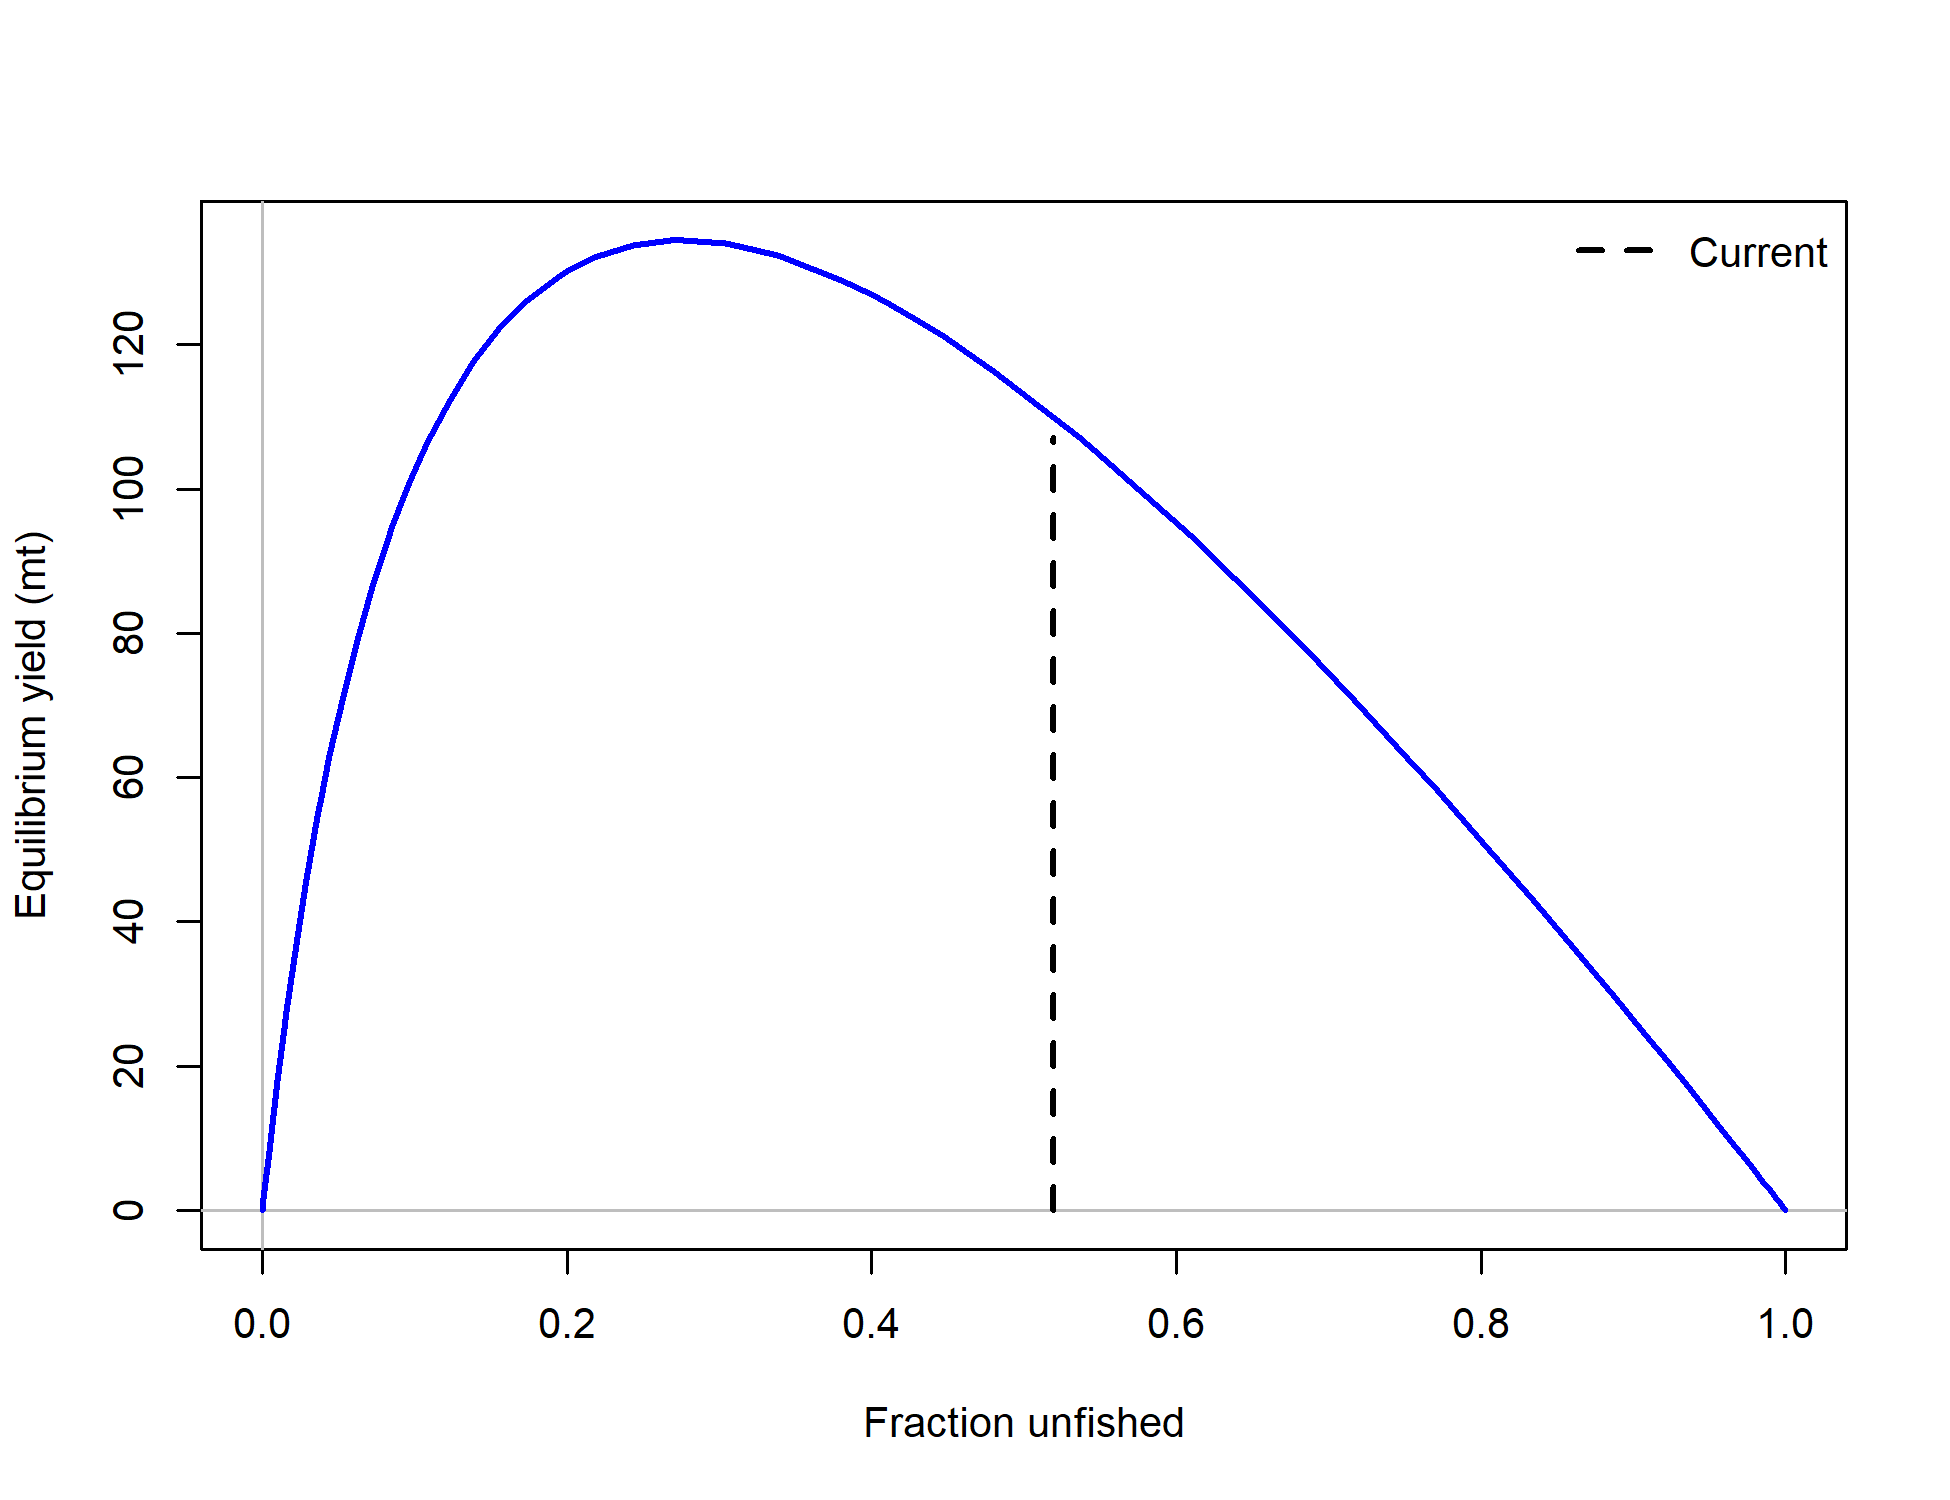
\includegraphics[width=1\textwidth,height=1\textheight]{N:/Assessments/CurrentAssessments/copper_rockfish_2023/models/nca/_bridging/2.4_dw/plots/yield2_yield_curve_with_refpoints.png}
\caption{Equilibrium yield curve for the base case model. Values are based on the 2020 fishery selectivities and with steepness fixed at 0.80.\label{fig:yield}}
\end{figure}

\hypertarget{detailed-fit-comps}{%
\section{Appendix A}\label{detailed-fit-comps}}

\hypertarget{detailed-fit-to-length-composition-data}{%
\subsection{Detailed Fit to Length Composition Data}\label{detailed-fit-to-length-composition-data}}

\hypertarget{detailed-fit-to-age-composition-data}{%
\subsection{Detailed Fit to Age Composition Data}\label{detailed-fit-to-age-composition-data}}

\hypertarget{detailed-fit-to-conditional-age-at-length-composition-data}{%
\subsection{Detailed Fit to Conditional-Age-at-Length Composition Data}\label{detailed-fit-to-conditional-age-at-length-composition-data}}

\hypertarget{mrfss-index}{%
\section{Appendix B. MRFSS Dockside Index of Abundance}\label{mrfss-index}}

\hypertarget{onboard-cpfv-index}{%
\section{Appendix C. California Onboard CPFV Index of Abundance}\label{onboard-cpfv-index}}

\hypertarget{dwv-cpfv-index}{%
\section{Appendix D. Deb Wilson-Vandenberg Onboard CPFV Index of Abundance}\label{dwv-cpfv-index}}

\hypertarget{crfs-pr-index}{%
\section{Appendix E. CRFS PR Dockside Index of Abundance}\label{crfs-pr-index}}

\hypertarget{ccfrp-index}{%
\section{Appendix F. CCFRP Index of Abundance}\label{ccfrp-index}}

\hypertarget{cdfw-rov-index}{%
\section{Appendix G. CDFW ROV Index of Abundance}\label{cdfw-rov-index}}

The California Department of Fish and Wildlife (CDFW) in collaboration with Marine Applied Research and Exploration (MARE) have been conducting remotely operated vehicle (ROV) surveys along the California coast in Marine Protected Areas (MPAs) and reference sites adjacent to them since 2004 for the purposes of long-term monitoring of changes in size, density (fish/square meter) and length of fish and invertebrate species along the California coast. Surveys of the entire coast have now been undertaken twice, each taking three years to complete, 2014-2016 and again in 2019-2021. The survey conducted multiple 500 meter transects across rocky reef survey sites. Sample sites were selected by first randomly selecting the deepest transect at a given site, then selecting transects on a constant interval into shallower depths. Transects were designed to be oriented parallel to general depth contours, though they were carried out using a fixed bearing that crossed depths in some cases.

Given that each pass of the California coast took a three year period, the STAT opted to explore using the data with super years. The selected super years were 2015 and 2020. Given the life history of copper rockfish an the limited movement of adult copper rockfish especially given the range of the survey area each year, the super year application was deemed reasonable in order to consider these data within the model. Minimal filtering were done to the data. Transects were removed based on four factors: 1) extreme estimates of effort (the estimated area of view below the ROV termed usable area), 2) any locations that were not sampled by both super year periods, 3) transect that were conducted across MPA and reference areas, and 4) transect conducted across depths that never observed copper rockfish within the survey (Table \ref{tab:rov-filtered}). Once the data were filtered the average calculated CPUE for each MPA and Reference groups were plotted to visualize the data (Table \ref{tab:rov-obs} and Figure \ref{fig:rov-raw-cpue}).

A range of alternative model structures were explored to generate an index of abundances including alternative error structures, covariates, and factors were considered when exploring how best to model these data. Based on model selection a model with super year, site designation (MPA or Reference), and super year site designation interaction was selected (Table \ref{tab:rov-model-selection}). A delta-lognormal model was selected based on the distribution of the data and diagnostics (Figure \ref{fig:rov-qq}) using sdmTMB (\textbf{anderson\_sdmtmb\_2022?}). The model estimates were then area-weighted based on the estimated percent of habitat within MPAs. An estimate of 8\% of rocky habitat within MPAs south of Point Conception and 92\% open to fishing were provided by John Budrick (CDFW). The estimated relative index of abundance is shown in Table \ref{tab:rov-index} and Figure \ref{fig:rov-index}.

\newpage

\begingroup\fontsize{10}{12}\selectfont
\begingroup\fontsize{10}{12}\selectfont

\begin{longtable}[t]{r>{\centering\arraybackslash}p{2cm}}
\caption{\label{tab:rov-filtered}Number of records filtered during data processing for the ROV survey data and the total remaining records.}\\
\toprule
Removal reason & Number\\
\midrule
\endfirsthead
\caption[]{Number of records filtered during data processing for the ROV survey data and the total remaining records. \textit{(continued)}}\\
\toprule
Removal reason & Number\\
\midrule
\endhead

\endfoot
\bottomrule
\endlastfoot
Records with usable area outside the 96th quantile & 38\\
Records with depths outside 19.3 - 99.8 m & 8\\
Rerence/MPA groups without sampling for both super years & 12\\
Retained records & 850\\*
\end{longtable}
\endgroup{}
\endgroup{}


\newpage

\begingroup\fontsize{7}{9}\selectfont

\begin{landscape}\begingroup\fontsize{7}{9}\selectfont

\begin{longtable}[t]{l>{\raggedright\arraybackslash}p{0.92cm}>{\raggedright\arraybackslash}p{0.92cm}>{\raggedright\arraybackslash}p{0.92cm}>{\raggedright\arraybackslash}p{0.92cm}>{\raggedright\arraybackslash}p{0.92cm}>{\raggedright\arraybackslash}p{0.92cm}>{\raggedright\arraybackslash}p{0.92cm}>{\raggedright\arraybackslash}p{0.92cm}>{\raggedright\arraybackslash}p{0.92cm}>{\raggedright\arraybackslash}p{0.92cm}>{\raggedright\arraybackslash}p{0.92cm}}
\caption{\label{tab:rov-model-selection}Model selection for the ROV survey.}\\
\toprule
Designation & Depth.Polynomial & Prop..Hard & Prop..Mixed & Prop..Soft & Super.Year & Designation.Super\_year & offset.log.usable.area. & DF & log.likelihood & AICc & Delta\\
\midrule
\endfirsthead
\caption[]{\label{tab:rov-model-selection}Model selection for the ROV survey. \textit{(continued)}}\\
\toprule
Designation & Depth.Polynomial & Prop..Hard & Prop..Mixed & Prop..Soft & Super.Year & Designation.Super\_year & offset.log.usable.area. & DF & log.likelihood & AICc & Delta\\
\midrule
\endhead

\endfoot
\bottomrule
\endlastfoot
+ & + & N.A. & N.A. & N.A. & + & + & + & 7 & -1257.3 & 2528.6 & 0.00\\
+ & + & N.A. & 0.45 & N.A. & + & + & + & 8 & -1256.3 & 2528.7 & 0.06\\
+ & + & -0.16 & N.A. & N.A. & + & + & + & 8 & -1257.0 & 2530.2 & 1.60\\
+ & + & N.A. & N.A. & -0.11 & + & + & + & 8 & -1257.2 & 2530.5 & 1.86\\
+ & + & N.A. & 0.46 & 0.02 & + & + & + & 9 & -1256.3 & 2530.7 & 2.10\\
+ & + & -0.02 & 0.44 & N.A. & + & + & + & 9 & -1256.3 & 2530.7 & 2.10\\
+ & + & -0.46 & N.A. & -0.44 & + & + & + & 9 & -1256.3 & 2530.7 & 2.10\\
+ & + & 12390456.41 & 12390456.86 & 12390456.42 & + & + & + & 10 & -1256.3 & 2532.8 & 4.13\\
+ & + & N.A. & 0.49 & N.A. & + & NA & + & 7 & -1260.4 & 2535.0 & 6.34\\
+ & + & N.A. & N.A. & N.A. & + & NA & + & 6 & -1261.6 & 2535.2 & 6.60\\
+ & + & -0.23 & N.A. & N.A. & + & NA & + & 7 & -1261.1 & 2536.3 & 7.71\\
+ & + & N.A. & 0.53 & 0.09 & + & NA & + & 8 & -1260.4 & 2536.9 & 8.25\\
+ & + & -0.09 & 0.44 & N.A. & + & NA & + & 8 & -1260.4 & 2536.9 & 8.25\\
+ & + & -0.53 & N.A. & -0.44 & + & NA & + & 8 & -1260.4 & 2536.9 & 8.25\\
+ & + & N.A. & N.A. & -0.05 & + & NA & + & 7 & -1261.5 & 2537.2 & 8.60\\
+ & + & 7762678.03 & 7762678.56 & 7762678.12 & + & NA & + & 9 & -1260.4 & 2538.9 & 10.29\\
+ & NA & -0.43 & N.A. & N.A. & + & + & + & 6 & -1271.3 & 2554.8 & 26.12\\
+ & NA & N.A. & 0.62 & 0.37 & + & + & + & 7 & -1271.1 & 2556.3 & 27.66\\
+ & NA & -0.37 & 0.24 & N.A. & + & + & + & 7 & -1271.1 & 2556.3 & 27.66\\
+ & NA & -0.62 & N.A. & -0.24 & + & + & + & 7 & -1271.1 & 2556.3 & 27.66\\
+ & NA & N.A. & N.A. & N.A. & + & + & + & 5 & -1273.2 & 2556.5 & 27.82\\
+ & NA & N.A. & 0.42 & N.A. & + & + & + & 6 & -1272.3 & 2556.8 & 28.15\\
+ & NA & N.A. & N.A. & 0.22 & + & + & + & 6 & -1272.7 & 2557.5 & 28.83\\
+ & NA & 14425294.28 & 14425294.89 & 14425294.65 & + & + & + & 8 & -1271.1 & 2558.3 & 29.67\\
+ & NA & -0.5 & N.A. & N.A. & + & NA & + & 5 & -1275.6 & 2561.2 & 32.62\\
+ & NA & N.A. & 0.69 & 0.44 & + & NA & + & 6 & -1275.3 & 2562.7 & 34.11\\
+ & NA & -0.44 & 0.25 & N.A. & + & NA & + & 6 & -1275.3 & 2562.7 & 34.11\\
+ & NA & -0.69 & N.A. & -0.25 & + & NA & + & 6 & -1275.3 & 2562.7 & 34.11\\
+ & NA & N.A. & 0.46 & N.A. & + & NA & + & 5 & -1277.0 & 2564.1 & 35.47\\
+ & NA & N.A. & N.A. & N.A. & + & NA & + & 4 & -1278.1 & 2564.2 & 35.52\\
+ & NA & N.A. & N.A. & 0.27 & + & NA & + & 5 & -1277.3 & 2564.7 & 36.07\\
+ & NA & 10396430.27 & 10396430.95 & 10396430.7 & + & NA & + & 7 & -1275.3 & 2564.8 & 36.13\\*
\end{longtable}
\endgroup{}
\end{landscape}
\endgroup{}

\newpage

\begingroup\fontsize{10}{12}\selectfont
\begingroup\fontsize{10}{12}\selectfont

\begin{longtable}[t]{c>{\centering\arraybackslash}p{2cm}>{\centering\arraybackslash}p{2cm}}
\caption{\label{tab:rov-index}Estimated relative index of abundance for the ROV survey.}\\
\toprule
Year & Estimate & logSE\\
\midrule
\endfirsthead
\caption[]{\label{tab:rov-index}Estimated relative index of abundance for the ROV survey. \textit{(continued)}}\\
\toprule
Year & Estimate & logSE\\
\midrule
\endhead

\endfoot
\bottomrule
\endlastfoot
2015 & 0.0248909 & 0.1359515\\
2020 & 0.0384396 & 0.0775755\\*
\end{longtable}
\endgroup{}
\endgroup{}

\newpage

\begin{figure}
\centering
\includegraphics[width=1\textwidth,height=1\textheight]{N:/Assessments/CurrentAssessments/copper_rockfish_2023/data/survey_indices/rov/delta_lognormal_north_designation_depth/qq.png}
\caption{QQ-plot for the ROV survey.\label{fig:rov-qq}}
\end{figure}

\newpage

\begin{figure}
\centering
\includegraphics[width=1\textwidth,height=1\textheight]{N:/Assessments/CurrentAssessments/copper_rockfish_2023/data/survey_indices/rov/delta_lognormal_north_designation_depth/Index.png}
\caption{The weighted relative index of abundance.\label{fig:rov-index}}
\end{figure}
\end{document}
